\documentclass[journal]{IEEEtran}
\usepackage{cite}
\usepackage{amsmath,amssymb,amsfonts,bm}
\usepackage{algorithm}
\usepackage{algpseudocode}
\usepackage{graphicx}
\usepackage{textcomp}
\usepackage{xcolor}
\usepackage{booktabs,multirow}
\usepackage{siunitx}
\usepackage[caption=false,font=footnotesize]{subfig}
\usepackage{tikz}
\usepackage{pgfplots,pgfplotstable}
\pgfplotsset{compat=1.18}
\usepgfplotslibrary{groupplots,fillbetween}
\usetikzlibrary{arrows.meta,positioning,fit,backgrounds,calc,shapes.geometric,shapes.misc}
\usepackage{url}
\usepackage[hidelinks]{hyperref}
\newtheorem{proposition}{Proposition}
\usepackage{etoolbox}
% IEEEtran hard-codes an em-dash after "Abstract" and "Index Terms"; replace it by a colon.
% The three hyphens are produced through \lowercase so that this file contains no triple hyphen.
\begingroup\lccode`\!=`\-
\lowercase{\endgroup
  \patchcmd{\abstract}{!!!}{:\ }{}{\PackageError{main}{abstract dash patch failed}{}}%
  \patchcmd{\IEEEkeywords}{!!!}{:\ }{}{\PackageError{main}{keywords dash patch failed}{}}%
}
\definecolor{cVITA}{HTML}{D55E00}\definecolor{cKM}{HTML}{0072B2}\definecolor{cKMed}{HTML}{56B4E9}
\definecolor{cHC}{HTML}{009E73}\definecolor{cHCX}{HTML}{CC79A7}\definecolor{cDP}{HTML}{E69F00}
\definecolor{cAE}{HTML}{6B6B6B}\definecolor{cCO}{HTML}{000000}\definecolor{cIX}{HTML}{8C564B}
\definecolor{cGrid}{HTML}{E6E6E6}\definecolor{cTint}{HTML}{F4F4F4}
\pgfplotsset{
  ieee/.style={width=\columnwidth, height=0.6\columnwidth, grid=major,
    major grid style={cGrid, line width=0.3pt}, axis line style={line width=0.5pt},
    tick style={line width=0.4pt}, label style={font=\footnotesize},
    tick label style={font=\scriptsize}, title style={font=\footnotesize},
    legend style={font=\scriptsize, draw=none, fill=none, legend cell align=left},
    every axis plot/.append style={line width=0.9pt, mark size=1.5pt}},
  m-VITA/.style={cVITA, line width=1.5pt, mark=*}, m-KM/.style={cKM, mark=square*},
  m-KMed/.style={cKMed, mark=diamond*}, m-HC/.style={cHC, mark=triangle*},
  m-HCX/.style={cHCX, mark=pentagon*}, m-DP/.style={cDP, mark=x},
  m-AE/.style={cAE, mark=o}, m-CO/.style={cCO, mark=star}, m-IX/.style={cIX, mark=+},
  m-FULL/.style={black, dashed, line width=0.8pt, mark=none}}

% generated by vita.export: do not edit
\newcommand{\AblBase}{0.474}
\newcommand{\AblBaseFive}{0.551}
\newcommand{\AblFive}{0.346}
\newcommand{\AblFour}{0.309}
\newcommand{\AblFull}{0.258}
\newcommand{\AblOne}{0.460}
\newcommand{\AblSix}{2.074}
\newcommand{\AblThree}{0.258}
\newcommand{\AblTwo}{0.536}
\newcommand{\BestBaseNameKeight}{KM}
\newcommand{\BestBaseNameKfour}{KM}
\newcommand{\BestBaseNameKsixteen}{KMed}
\newcommand{\BestIterMean}{0.3}
\newcommand{\CFVitaSmallMax}{1.08}
\newcommand{\CFVitaSmallMin}{0.61}
\newcommand{\COErrBestBaseKeight}{0.49}
\newcommand{\COErrBestBaseKfour}{2.67}
\newcommand{\COErrBestBaseKsixteen}{0.41}
\newcommand{\COErrVITAKeight}{0.73}
\newcommand{\COErrVITAKfour}{1.84}
\newcommand{\COErrVITAKsixteen}{0.68}
\newcommand{\CapDevBaseName}{KM}
\newcommand{\CapDevBatEBase}{0.24}
\newcommand{\CapDevBatEVITA}{0.43}
\newcommand{\CapDevBestBaseKeight}{5.0}
\newcommand{\CapDevBestBaseKfour}{10.3}
\newcommand{\CapDevBestBaseKsixteen}{3.2}
\newcommand{\CapDevPVBase}{1.28}
\newcommand{\CapDevPVVITA}{0.92}
\newcommand{\CapDevQHBase}{0.46}
\newcommand{\CapDevQHVITA}{0.15}
\newcommand{\CapDevVITAKeight}{10.2}
\newcommand{\CapDevVITAKfour}{14.7}
\newcommand{\CapDevVITAKsixteen}{6.9}
\newcommand{\CapDevWindBase}{0.44}
\newcommand{\CapDevWindVITA}{1.16}
\newcommand{\CorrSOCBase}{0.85}
\newcommand{\CorrSOCVITA}{0.23}
\newcommand{\CostErrBestBaseKeight}{7.22}
\newcommand{\CostErrBestBaseKfour}{13.44}
\newcommand{\CostErrBestBaseKsixteen}{3.10}
\newcommand{\CostErrVITAKeight}{9.95}
\newcommand{\CostErrVITAKfour}{14.90}
\newcommand{\CostErrVITAKsixteen}{7.98}
\newcommand{\DataRows}{35{,}064}
\newcommand{\DegenDualPct}{100.0}
\newcommand{\DegenPrimalPct}{100.0}
\newcommand{\DegenSampled}{8525}
\newcommand{\DevBestBaseKeight}{0.255}
\newcommand{\DevBestBaseKsixteen}{0.092}
\newcommand{\DevBestBaseNameKeight}{KMed}
\newcommand{\DevBestBaseNameKsixteen}{KMed}
\newcommand{\DevTargetKeight}{0.217}
\newcommand{\DevTargetKsixteen}{0.092}
\newcommand{\DevVITAKeight}{0.683}
\newcommand{\DevVITAKsixteen}{0.393}
\newcommand{\DevVITAMaxKeight}{0.950}
\newcommand{\DevVITAMaxKsixteen}{0.494}
\newcommand{\DevVITAMinKeight}{0.203}
\newcommand{\DevVITAMinKsixteen}{0.262}
\newcommand{\FigFiveStorage}{thermal tank}
\newcommand{\FigFiveSwing}{194}
\newcommand{\FigFiveYear}{2018}
\newcommand{\FigThreeYmax}{10}
\newcommand{\FigThreeYmin}{0.05}
\newcommand{\FilledPVTotal}{18}
\newcommand{\FilledWindTotal}{18}
\newcommand{\FullOperTimeMean}{3.6}
\newcommand{\GradSharePV}{24.0}
\newcommand{\GradSharePrice}{3.5}
\newcommand{\GradShareWeekday}{66.3}
\newcommand{\GradShareWind}{6.2}
\newcommand{\MaxRegBase}{13.8}
\newcommand{\MaxRegBaseName}{IX}
\newcommand{\MaxRegVITA}{29.2}
\newcommand{\MaxRegVITAK}{4}
\newcommand{\MaxRegVITAPrice}{250}
\newcommand{\MaxRegVITAUnserved}{0.39}
\newcommand{\MaxRegVITAYear}{2016}
\newcommand{\MedianRegBestKeight}{0.241}
\newcommand{\MedianRegVITAKeight}{0.566}
\newcommand{\MedianRegVITAKeightInst}{0.566}
\newcommand{\MedianRegVITAKfourInst}{1.376}
\newcommand{\MedianRegVITAKsixteenInst}{0.338}
\newcommand{\MinPHolmKeight}{0.055}
\newcommand{\MinPHolmKsixteen}{0.008}
\newcommand{\NAllEvals}{396}
\newcommand{\NBaseEvals}{288}
\newcommand{\NCatBase}{12}
\newcommand{\NCatVITA}{1}
\newcommand{\NDaysMixedKM}{9}
\newcommand{\NDaysMixedVITA}{113}
\newcommand{\NInitSelected}{18}
\newcommand{\NMixedKM}{1}
\newcommand{\NMixedVITA}{2}
\newcommand{\NRuns}{36}
\newcommand{\NSigBetterKeight}{0}
\newcommand{\NSigBetterKsixteen}{0}
\newcommand{\NSigWorseKeight}{0}
\newcommand{\NSigWorseKsixteen}{1}
\newcommand{\NTest}{12}
\newcommand{\NUnservedEvals}{3}
\newcommand{\NVITAEvals}{108}
\newcommand{\NVitaSmall}{3}
\newcommand{\OracleCOEighty}{8.7}
\newcommand{\OracleCOOneFifty}{0.2}
\newcommand{\OracleCOTwoFifty}{0.0}
\newcommand{\OracleNoCOEighty}{0}
\newcommand{\OracleNoCOOneFifty}{3}
\newcommand{\OracleNoCOTwoFifty}{4}
\newcommand{\OracleQHEighty}{10.0}
\newcommand{\OracleQHOneFifty}{29.0}
\newcommand{\OracleQHTwoFifty}{30.0}
\newcommand{\OracleQebEighty}{20.0}
\newcommand{\OracleQebOneFifty}{1.0}
\newcommand{\OracleQebTwoFifty}{0.0}
\newcommand{\OracleQgbEighty}{20.0}
\newcommand{\OracleQgbOneFifty}{1.0}
\newcommand{\OracleQgbTwoFifty}{0.0}
\newcommand{\OracleTimeMedian}{454}
\newcommand{\PHolmBestKeight}{0.055}
\newcommand{\PHolmBestKsixteen}{0.008}
\newcommand{\RegAEKeight}{0.536}
\newcommand{\RegAEKfour}{1.737}
\newcommand{\RegAEKsixteen}{0.377}
\newcommand{\RegBestBaseKeight}{0.295}
\newcommand{\RegBestBaseKfour}{0.779}
\newcommand{\RegBestBaseKsixteen}{0.117}
\newcommand{\RegCOKeight}{0.658}
\newcommand{\RegCOKfour}{3.843}
\newcommand{\RegCOKsixteen}{0.312}
\newcommand{\RegDPKeight}{0.581}
\newcommand{\RegDPKfour}{1.053}
\newcommand{\RegDPKsixteen}{0.453}
\newcommand{\RegHCKeight}{0.450}
\newcommand{\RegHCKeightEighty}{0.220}
\newcommand{\RegHCKeightOneFifty}{0.569}
\newcommand{\RegHCKeightTwoFifty}{0.562}
\newcommand{\RegHCKfour}{2.505}
\newcommand{\RegHCKsixteen}{0.400}
\newcommand{\RegHCXKeight}{0.754}
\newcommand{\RegHCXKfour}{3.792}
\newcommand{\RegHCXKsixteen}{0.382}
\newcommand{\RegIXKeight}{0.917}
\newcommand{\RegIXKfour}{6.289}
\newcommand{\RegIXKsixteen}{0.339}
\newcommand{\RegKMKeight}{0.295}
\newcommand{\RegKMKeightEighty}{0.316}
\newcommand{\RegKMKeightOneFifty}{0.301}
\newcommand{\RegKMKeightTwoFifty}{0.267}
\newcommand{\RegKMKfour}{0.779}
\newcommand{\RegKMKsixteen}{0.259}
\newcommand{\RegKMedKeight}{0.437}
\newcommand{\RegKMedKeightEighty}{0.370}
\newcommand{\RegKMedKeightOneFifty}{0.474}
\newcommand{\RegKMedKeightTwoFifty}{0.467}
\newcommand{\RegKMedKfour}{0.836}
\newcommand{\RegKMedKsixteen}{0.117}
\newcommand{\RegSdVITAKeight}{0.753}
\newcommand{\RegSdVITAKfour}{4.725}
\newcommand{\RegSdVITAKsixteen}{0.453}
\newcommand{\RegVITAKeight}{0.800}
\newcommand{\RegVITAKeightEighty}{0.607}
\newcommand{\RegVITAKeightOneFifty}{0.886}
\newcommand{\RegVITAKeightTwoFifty}{0.906}
\newcommand{\RegVITAKfour}{2.081}
\newcommand{\RegVITAKsixteen}{0.494}
\newcommand{\RuntimeBestBaseKeight}{0.68}
\newcommand{\RuntimeBestBaseKfour}{0.26}
\newcommand{\RuntimeBestBaseKsixteen}{2.13}
\newcommand{\RuntimeIXKeight}{19.3}
\newcommand{\RuntimeVITAKeight}{0.45}
\newcommand{\RuntimeVITAKfour}{0.17}
\newcommand{\RuntimeVITAKsixteen}{1.40}
\newcommand{\SOCBaseMon}{157}
\newcommand{\SOCBaseSat}{27}
\newcommand{\SOCFullMon}{153}
\newcommand{\SOCFullSat}{20}
\newcommand{\SOCVITAMon}{120}
\newcommand{\SOCVITASat}{80}
\newcommand{\SatTauEnd}{96.7}
\newcommand{\SatTauLate}{76.7}
\newcommand{\SatTauOne}{36.2}
\newcommand{\SpeedupKeight}{1014}
\newcommand{\TrainTimeKeight}{5.6}
\newcommand{\TrainTimeKfour}{3.4}
\newcommand{\TrainTimeKsixteen}{12.3}
\newcommand{\UnservedBestBaseKeight}{0.0000}
\newcommand{\UnservedBestBaseKfour}{0.0000}
\newcommand{\UnservedBestBaseKsixteen}{0.0000}
\newcommand{\UnservedVITAKeight}{0.0000}
\newcommand{\UnservedVITAKfour}{0.0108}
\newcommand{\UnservedVITAKsixteen}{0.0000}
\newcommand{\VITASeedMaxKeight}{1.261}
\newcommand{\VITASeedMinKeight}{0.258}
\newcommand{\VITAYearMaxKeight}{1.701}
\newcommand{\VITAYearMinKeight}{0.285}
\newcommand{\WKMMax}{77}
\newcommand{\WKMMin}{9}
\newcommand{\WVitaTopThree}{287}
\newcommand{\WinsVsBestKeight}{3}
\newcommand{\WinsVsBestKsixteen}{1}

\markboth{}{Bahi: Value-Informed Neural Temporal Aggregation for Sector-Coupled Industrial Energy Hubs}

\begin{document}
\bstctlcite{IEEEexample:BSTcontrol}% disables the dash that IEEEtran.bst prints for repeated author lists
\title{Value-Informed Neural Temporal Aggregation for the Design of Sector-Coupled Industrial Energy Hubs}
\author{Abderaouf~Bahi%
\thanks{A. Bahi is with the LIMA Laboratory, Chadli Bendjedid El Tarf University, El Tarf, Algeria (e-mail: a.bahi@univ-eltarf.dz).}}
\maketitle
\begin{abstract}
Sizing sector-coupled industrial energy hubs, which electrify process heat, produce hydrogen and add renewables and storage, requires hourly operation over full years. Time-series aggregation makes these design models tractable, but classical aggregation clusters input profiles without regard to the resulting design, and decision-aware alternatives need full-resolution solves for every new instance. This paper proposes value-informed temporal aggregation (VITA), a neural aggregation map trained to match the value function and subgradients of the aggregated operational model to those of the full-resolution model on candidate designs. Exact gradients follow from linear programming duality, a regret bound motivates the loss, and deployment needs no full-resolution solve. VITA is benchmarked against eight aggregation methods on a hub with electricity, two heat levels and hydrogen, using Spanish data for 2015 to 2018, leave-one-year-out testing and three carbon prices, with every design evaluated at full resolution. VITA reached a mean test regret of \RegVITAKeight\,\% at eight representative days and \RegVITAKsixteen\,\% at sixteen, against \RegBestBaseKeight\,\% and \RegBestBaseKsixteen\,\% for the best baselines (\BestBaseNameKeight{} and \BestBaseNameKsixteen{}). Diagnostics show that the value-matching gradient acts mainly on the weekday share of representative days (\GradShareWeekday\,\% of its norm), a quantity that real days cannot take fractionally, and that the soft assignment saturates during training. Clustering standardized inputs with medoids or centroids remained the most reliable choice; decision-focused aggregation needs offset-invariant objectives and representations that preserve binary demand drivers.
\end{abstract}

\begin{IEEEkeywords}
Capacity expansion planning, decision-focused learning, energy hub, industrial decarbonization, linear programming duality, sector coupling, time-series aggregation.
\end{IEEEkeywords}

\section{Introduction}
\IEEEPARstart{I}{ndustrial} sites account for a large share of final energy use and of direct CO$_2$ emissions, and most of their energy demand is process heat~\cite{rissman2020industry}. Deep decarbonization of such sites combines several levers at once: process heat is electrified with industrial heat pumps and electric boilers, hydrogen feedstock is produced on site by electrolysis, and on-site photovoltaics, wind turbines and storage reduce the cost of the electricity that all these converters draw from the grid. The resulting plant is a sector-coupled energy hub~\cite{geidl2007energyhubs,mancarella2014mes} in which electricity, heat at several temperature levels and hydrogen interact through converters and storage. Sizing it is a capacity expansion problem whose operating part must be represented at hourly resolution over full years, because day-ahead prices, renewable availability and heat demand vary on time scales that range from hours to seasons, and because storage couples these time scales~\cite{gabrielli2018seasonal,brown2018synergies}.

A single-node linear design model of such a hub with one year of hourly operation already has about $2\times 10^{5}$ variables and constraints. The full-resolution model becomes intractable as soon as networks, several weather years, uncertainty scenarios or integer sizing decisions are added, so planners resort to time-series aggregation (TSA): a year is replaced by $K$ weighted representative days, and storage that shifts energy between days is handled by linking the representative days through the chronological sequence of the year~\cite{kotzur2018seasonal,pineda2018chronological}. Reviews of the field~\cite{hoffmann2020review,teichgraeber2022review} recommend that TSA be judged on the quality of the optimization outcome, validated on the full time series, rather than on the statistical fidelity of the aggregated profiles.

Classical TSA clusters the input profiles and ignores the downstream decision~\cite{kotzur2018impact,teichgraeber2019clustering}. Statistical fidelity of the representative days does not imply good designs: a cluster centroid can average away a demand peak that sizes a converter, and a medoid can misrepresent the energy content of its cluster. Decision-aware alternatives either evaluate candidate aggregations against the full-resolution model for every new instance, as in iterative extreme-period selection~\cite{teichgraeber2021iterative}, a posteriori aggregation~\cite{hilbers2023aposteriori} and duality-based exact aggregation~\cite{santosuosso2026marginal,rybka2026mlexact}, or cluster on hand-crafted decision features such as the designs of single-day models~\cite{sun2019costoriented,zhang2023modeladaptive}. Learned approaches compress the input data with autoencoders before clustering~\cite{barbar2022autoencoder}, but the encoder is not trained on the quality of the resulting design. Decision-focused learning~\cite{elmachtoub2022spo,mandi2024dfl} trains predictive models through the optimization problems that consume their output; it has not been used to learn the aggregation itself.

This paper closes that gap with VITA (value-informed temporal aggregation), a neural aggregation map trained on the decisions it induces. A convolutional encoder embeds each day, learnable prototypes assign days softly to clusters, and the representative days and weights are soft cluster means and masses of real days. Training matches the value function of the aggregated operational model to the value function of the full-resolution operational model on a set of candidate designs, together with its first-order behavior given by linear programming (LP) duals. Gradients through the aggregated LP are exact and inexpensive because, by LP sensitivity theory, they follow from the optimal primal and dual solutions returned by the solver. Once trained, VITA aggregates a new year in one forward pass and needs no full-resolution solve (Fig.~\ref{fig:pipeline}). The contributions are:

\begin{figure*}[!t]
\centering
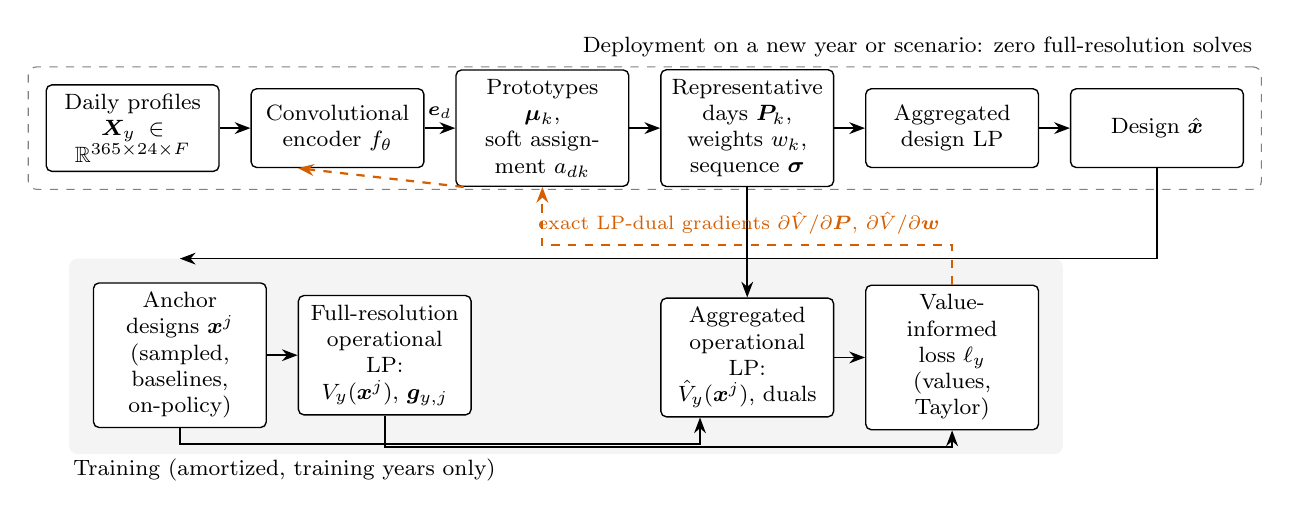
\begin{tikzpicture}[
  font=\footnotesize,
  box/.style={draw, rounded corners=2pt, align=center, minimum height=10mm, text width=19.6mm, line width=0.5pt, fill=white},
  arr/.style={-{Stealth[length=2mm]}, line width=0.6pt},
  grad/.style={-{Stealth[length=2mm]}, dashed, line width=0.8pt, cVITA},
  node distance=4.5mm and 3.9mm]
\node[box] (X) {Daily profiles\\ $\bm{X}_y\in\mathbb{R}^{365\times24\times F}$};
\node[box, right=of X] (E) {Convolutional\\ encoder $f_{\theta}$};
\node[box, right=of E] (A) {Prototypes $\bm{\mu}_k$,\\ soft assignment $a_{dk}$};
\node[box, right=of A] (P) {Representative days $\bm{P}_k$,\\ weights $w_k$, sequence $\bm{\sigma}$};
\node[box, right=of P] (L) {Aggregated\\ design LP};
\node[box, right=of L] (D) {Design $\hat{\bm{x}}$};
\draw[arr] (X) -- (E);
\draw[arr] (E) -- node[above, font=\scriptsize]{$\bm{e}_d$} (A);
\draw[arr] (A) -- (P);
\draw[arr] (P) -- (L);
\draw[arr] (L) -- (D);
% training loop
\node[box, below=14mm of X, xshift=6mm] (J) {Anchor designs $\bm{x}^{j}$\\ (sampled, baselines,\\ on-policy)};
\node[box, right=of J] (F) {Full-resolution\\ operational LP:\\ $V_y(\bm{x}^{j})$, $\bm{g}_{y,j}$};
\node[box, below=14mm of P] (O) {Aggregated\\ operational LP:\\ $\hat{V}_y(\bm{x}^{j})$, duals};
\node[box, right=of O] (Lo) {Value-informed\\ loss $\ell_y$\\ (values, Taylor)};
\draw[arr] (J) -- (F);
\draw[arr] (P) -- (O);
\draw[arr] (O) -- (Lo);
\draw[arr] (F.south) -- ++(0,-4mm) -| (Lo.south);
\draw[arr] (J.south) -- ++(0,-2mm) -| ([xshift=-6mm]O.south);
\draw[arr] (D.south) |- ([yshift=3mm]J.north east) -- ([yshift=3mm]J.north);
\draw[grad] (Lo.north) -- ++(0,5mm) -| node[pos=0.26, above, font=\scriptsize]{exact LP-dual gradients $\partial\hat{V}/\partial\bm{P},\,\partial\hat{V}/\partial\bm{w}$} (A.south);
\draw[grad] ([xshift=5mm]A.south) ++(-15mm,0) -- ([xshift=-5mm]E.south);
\begin{scope}[on background layer]
\node[fit=(J)(F)(O)(Lo), fill=cTint, rounded corners=3pt, inner sep=3mm, ] (trainbox) {};
\node[font=\footnotesize, anchor=north west, inner sep=1.5pt] at (trainbox.south west) {Training (amortized, training years only)};
\node[fit=(X)(D), draw=black!50, dashed, rounded corners=3pt, inner sep=2.2mm, label={[font=\footnotesize, anchor=south east]north east:Deployment on a new year or scenario: zero full-resolution solves}] {};
\end{scope}
\end{tikzpicture}
\caption{VITA trains a neural aggregation map on the value of the decisions it induces and deploys it without any full-resolution solve. Solid arrows show the forward pipeline from daily profiles to a design; the tinted box shows training, in which the aggregated operational value is matched to the full-resolution value and its subgradient at anchor designs; dashed vermillion arrows show the exact gradients obtained from LP duals.}
\label{fig:pipeline}
\end{figure*}


\begin{enumerate}
\item VITA, a decision-focused neural TSA method for sector-coupled design models, trained on value-function and dual-informed Taylor targets, with a regret bound that motivates the loss.
\item Exact, solver-agnostic gradients of the aggregated model through LP duality, including inter-period storage linking for long-duration storage, implemented as a custom automatic differentiation operator with warm-started solver instances and verified against finite differences.
\item A sector-coupled industrial hub model (electricity, low- and high-temperature heat, hydrogen) and an open benchmark against eight TSA baselines in which every design is evaluated with the full-resolution model.
\item Evidence on zero-shot transfer to unseen years and carbon-price scenarios, and an analysis of how aggregation errors distort decarbonization investment decisions.
\end{enumerate}

Section~\ref{sec:related} reviews related work, Section~\ref{sec:problem} states the design problem, Section~\ref{sec:method} presents VITA, Section~\ref{sec:setup} describes the case study, Section~\ref{sec:results} reports the results and Section~\ref{sec:conclusion} concludes.

\section{Related Work}\label{sec:related}

\subsection{Design of Multi-Energy and Sector-Coupled Systems}
Multi-energy systems couple carriers through conversion and storage so that the flexibility of one carrier serves the others~\cite{mancarella2014mes}. The energy hub abstraction describes such systems as buses linked by converters with fixed or time-varying efficiencies~\cite{geidl2007energyhubs}, and it underlies most design models of districts and industrial parks. Optimal design of multi-energy systems with seasonal storage requires the operation of a whole year, because storage shifts energy across seasons and couples days~\cite{gabrielli2018seasonal}. At the continental scale, sector coupling of heat and transport with electricity lowers system cost and shifts the value of flexibility between options~\cite{brown2018synergies}. For industry, electrified process heat, hydrogen and on-site renewables are among the main mitigation routes~\cite{rissman2020industry}, which makes the industrial hub studied here a representative design problem of the energy transition.

\subsection{Time-Series Aggregation}
Reviews~\cite{hoffmann2020review,teichgraeber2022review} classify TSA by the clustering algorithm, the representation of each cluster and the treatment of inter-period dynamics. Statistical TSA clusters daily input vectors with k-means, k-medoids or hierarchical algorithms and represents clusters by centroids or medoids~\cite{kotzur2018impact,teichgraeber2019clustering}; representative days can also be selected by optimization to reproduce duration curves~\cite{poncelet2017selecting}. Extreme periods are added to preserve peaks~\cite{kotzur2018impact}, and distribution-preserving representations reproduce the value distribution of each cluster~\cite{hoffmann2022pareto}. Long-duration storage requires linking representative periods through the chronological sequence of the year, either by chronological clustering~\cite{pineda2018chronological} or by the superposition of intra- and inter-period states~\cite{kotzur2018seasonal}, which this paper adopts.

Decision-aware methods use information from the optimization model. Cost-oriented selection clusters days by the designs of single-day models~\cite{sun2019costoriented}, and model-adaptive clustering extracts features from the energy system model~\cite{zhang2023modeladaptive}. Iterative extreme-period selection adds the periods in which a design fails when operated over the full year~\cite{teichgraeber2021iterative}, and a posteriori aggregation adapts the aggregation to the model with storage through full-horizon evaluation~\cite{hilbers2023aposteriori}. A duality-based line of work shows that aggregation is exact when it preserves the active constraints of the full model~\cite{wogrin2023onesize}, extends the idea to network and ramping constraints~\cite{cardonavasquez2024enhancing}, and uses estimated marginal costs as clustering features in iterative schemes with performance bounds~\cite{santosuosso2026marginal,rybka2026mlexact}. These methods require full-resolution or fixed-design full-horizon solves for every new instance. Learned TSA embeds periods with autoencoders before clustering~\cite{barbar2022autoencoder}; the embedding is trained for reconstruction and is not informed by the design quality. Table~\ref{tab:positioning} summarizes the positioning.

\begin{table}[!t]
\centering
\caption{Positioning of VITA Against Representative TSA Families\label{tab:positioning}}
\footnotesize
\setlength{\tabcolsep}{1.6pt}
\begin{tabular}{@{}lcccc@{}}
\toprule
Family & Model & Neural & Trained on & Full solves \\
 & information & features & decisions & per instance \\
\midrule
Statistical~\cite{kotzur2018impact,teichgraeber2019clustering} & no & no & no & no \\
Extreme periods~\cite{kotzur2018impact} & no & no & no & no \\
Distribution~\cite{hoffmann2022pareto} & no & no & no & no \\
Cost oriented~\cite{sun2019costoriented} & yes & no & no & no \\
Iterative extremes~\cite{teichgraeber2021iterative} & yes & no & no & yes \\
A posteriori~\cite{hilbers2023aposteriori} & yes & no & no & yes \\
Marginal-cost TSA~\cite{santosuosso2026marginal} & yes & no & no & yes \\
ML marginal costs~\cite{rybka2026mlexact} & yes & n/a & no & yes \\
Autoencoder~\cite{barbar2022autoencoder} & yes & yes & no & no \\
VITA (this paper) & yes & yes & yes & no \\
\bottomrule
\end{tabular}
\end{table}

\subsection{Decision-Focused Learning and Differentiable Optimization}
Decision-focused learning trains a predictor through the optimization problem that consumes its output, so that the loss reflects decision quality rather than prediction accuracy~\cite{mandi2024dfl}. The smart predict-then-optimize loss gives a convex surrogate of decision regret for linear objectives~\cite{elmachtoub2022spo}, task-based learning differentiates through stochastic programs~\cite{donti2017taskbased}, and differentiable optimization layers backpropagate through the Karush-Kuhn-Tucker conditions of quadratic programs~\cite{amos2017optnet}. In energy systems, wind power forecasts trained end to end on system cost outperform accuracy-trained forecasts~\cite{wahdany2023morethan}. VITA transfers this idea from forecasting to aggregation: the learned object is the map from a year of data to a reduced model, and the decision loss is computed with a value function rather than with a single downstream decision. Because the aggregated model is an LP, exact sensitivities follow from the primal and dual solutions of a simplex solver~\cite{huangfu2018highs}, without a differentiable solver layer.

\section{Problem Formulation}\label{sec:problem}

\subsection{Sector-Coupled Industrial Hub}
The hub of Fig.~\ref{fig:hub} has four buses: electricity, low-temperature (LT) heat, high-temperature (HT) process heat (steam) and hydrogen. Electricity is supplied by grid imports, photovoltaics (PV), onshore wind and a battery; LT heat by an air-source heat pump, heat recovered from the electrolyzer and a thermal water tank; HT heat by an industrial heat pump that upgrades waste heat, an electric boiler and a gas boiler; hydrogen by an electrolyzer and a pressurized tank. The design vector $\bm{x}\in\mathbb{R}^{11}_{\ge 0}$ collects the capacities of PV ($P^{\mathrm{pv}}$), wind ($P^{\mathrm{wd}}$), battery energy and power ($E^{\mathrm{bat}}$, $P^{\mathrm{bat}}$), electrolyzer ($P^{\mathrm{ely}}$), hydrogen tank ($E^{\mathrm{h2}}$), LT and HT heat pumps ($Q^{\mathrm{L}}$, $Q^{\mathrm{H}}$), electric and gas boilers ($Q^{\mathrm{eb}}$, $Q^{\mathrm{gb}}$) and thermal tank ($E^{\mathrm{tes}}$). Each capacity has an annualized capital cost $\kappa_i$ (capital recovery factor plus fixed operation and maintenance).

\begin{figure}[!t]
\centering
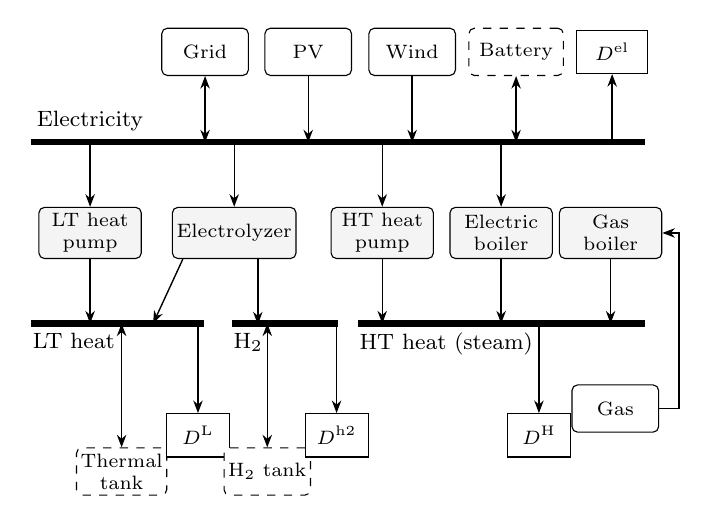
\begin{tikzpicture}[
  font=\scriptsize,
  src/.style={draw, rounded corners=2pt, align=center, minimum height=6mm, minimum width=11mm, inner sep=1.5pt, fill=white},
  conv/.style={draw, rounded corners=2pt, align=center, minimum height=6.5mm, minimum width=13mm, inner sep=1.5pt, fill=cTint},
  sto/.style={draw, rounded corners=2pt, align=center, minimum height=6mm, minimum width=12mm, inner sep=1.5pt, fill=white, dashed},
  dem/.style={draw, align=center, minimum height=5.5mm, minimum width=9mm, inner sep=1.5pt, fill=white},
  bus/.style={line width=2.2pt},
  arr/.style={-{Stealth[length=1.6mm]}, line width=0.5pt},
  barr/.style={{Stealth[length=1.6mm]}-{Stealth[length=1.6mm]}, line width=0.5pt}]
% electricity bus
\draw[bus] (0.00,3.6) -- (7.80,3.6) node[pos=0, above right=0.5pt, font=\scriptsize\bfseries]{};
\node[anchor=south west, font=\footnotesize] at (-0.05,3.62) {Electricity};
\node[src] (grid) at (2.21,4.75) {Grid};
\node[src] (pv) at (3.52,4.75) {PV};
\node[src] (wd) at (4.84,4.75) {Wind};
\node[sto] (bat) at (6.16,4.75) {Battery};
\node[dem] (del) at (7.38,4.75) {$D^{\mathrm{el}}$};
\draw[barr] (grid) -- (grid|-0,3.6);
\draw[arr] (pv) -- (pv|-0,3.6);
\draw[arr] (wd) -- (wd|-0,3.6);
\draw[barr] (bat) -- (bat|-0,3.6);
\draw[arr] (del|-0,3.6) -- (del);
% converters
\node[conv] (hpl) at (0.75,2.45) {LT heat\\ pump};
\node[conv] (ely) at (2.58,2.45) {Electrolyzer};
\node[conv] (hph) at (4.46,2.45) {HT heat\\ pump};
\node[conv] (eb) at (5.97,2.45) {Electric\\ boiler};
\draw[arr] (hpl|-0,3.6) -- (hpl);
\draw[arr] (ely|-0,3.6) -- (ely);
\draw[arr] (hph|-0,3.6) -- (hph);
\draw[arr] (eb|-0,3.6) -- (eb);
% heat and hydrogen buses
\draw[bus] (0,1.3) -- (2.2,1.3);
\node[anchor=north west, font=\footnotesize, inner sep=1pt] at (-0.02,1.22) {LT heat};
\draw[bus] (2.55,1.3) -- (3.9,1.3);
\node[anchor=north west, font=\footnotesize, inner sep=1pt] at (2.53,1.22) {H$_2$};
\draw[bus] (4.15,1.3) -- (7.8,1.3);
\node[anchor=north west, font=\footnotesize, inner sep=1pt] at (4.13,1.22) {HT heat (steam)};
\draw[arr] (hpl) -- (hpl|-0,1.3);
\draw[arr] (ely.south) ++(0.3,0) -- ++(0,-0.83);
\draw[arr] (ely.south west) ++(0.14,0) -- (1.55,1.3);
\draw[arr] (hph) -- (hph|-0,1.3);
\draw[arr] (eb) -- (eb|-0,1.3);
\node[conv] (gb) at (7.36,2.45) {Gas\\ boiler};
\node[src] (gas) at (7.42,0.22) {Gas};
\draw[arr] (gb) -- (gb|-0,1.3);
\draw[arr] (gas.east) -- ++(0.25,0) |- (gb.east);
% storages and demands
\node[sto, minimum width=10mm] (tes) at (1.15,-0.58) {Thermal\\ tank};
\node[dem, minimum width=8mm] (dl) at (2.12,-0.12) {$D^{\mathrm{L}}$};
\node[sto, minimum width=9.5mm] (h2t) at (3.0,-0.58) {H$_2$ tank};
\node[dem, minimum width=8mm] (dh2) at (3.88,-0.12) {$D^{\mathrm{h2}}$};
\node[dem, minimum width=8mm] (dh) at (6.45,-0.12) {$D^{\mathrm{H}}$};
\draw[barr] (tes) -- (tes|-0,1.3);
\draw[arr] (dl|-0,1.3) -- (dl);
\draw[barr] (h2t) -- (h2t|-0,1.3);
\draw[arr] (dh2|-0,1.3) -- (dh2);
\draw[arr] (dh|-0,1.3) -- (dh);
\end{tikzpicture}
\caption{The industrial hub couples electricity, low-temperature heat, high-temperature process heat and hydrogen through five converters and three storages. Shaded boxes are converters, dashed boxes are storages and plain boxes on the buses are demands; the electrolyzer feeds hydrogen and recovered heat.}
\label{fig:hub}
\end{figure}


\subsection{Full-Resolution Design Model}
For a year $y$ with hours $t=1,\dots,T$ ($T=8760$), the operating variables are grid import and export $g^{+}_t,g^{-}_t$, PV and wind output $p^{\mathrm{pv}}_t,p^{\mathrm{wd}}_t$, battery charge, discharge and state $b^{+}_t,b^{-}_t,s^{\mathrm{b}}_t$, electrolyzer input $e_t$ and recovered heat $r_t$, hydrogen injection, withdrawal and state $h^{+}_t,h^{-}_t,s^{\mathrm{h}}_t$, converter outputs $q^{\mathrm{L}}_t,q^{\mathrm{H}}_t,q^{\mathrm{eb}}_t,q^{\mathrm{gb}}_t$, thermal tank charge, discharge and state $z^{+}_t,z^{-}_t,s^{\mathrm{z}}_t$, and unserved energy $u^{c}_t$ for each carrier $c\in\{\mathrm{el},\mathrm{L},\mathrm{H},\mathrm{h2}\}$. The design LP reads
\begin{align}
\min\;& \bm{\kappa}^{\top}\bm{x}+\sum_{t}\Big[(\pi_t+\phi^{+})g^{+}_t-(\pi_t-\phi^{-})g^{-}_t+c^{\mathrm{gb}}q^{\mathrm{gb}}_t \nonumber\\
&\qquad\qquad +\bm{c}^{\mathrm{vom}\top}\bm{q}_t+c^{u}\textstyle\sum_{c}u^{c}_t\Big] \label{eq:obj}\\
\text{s.t. }& p^{\mathrm{pv}}_t+p^{\mathrm{wd}}_t+g^{+}_t+b^{-}_t+u^{\mathrm{el}}_t = D^{\mathrm{el}}_t+g^{-}_t+b^{+}_t+e_t \nonumber\\
&\qquad +q^{\mathrm{L}}_t/\mathrm{COP}^{\mathrm{L}}_t+q^{\mathrm{H}}_t/\mathrm{COP}^{\mathrm{H}}+q^{\mathrm{eb}}_t/\eta^{\mathrm{eb}}, \label{eq:el}\\
& q^{\mathrm{L}}_t+r_t+z^{-}_t-z^{+}_t+u^{\mathrm{L}}_t=D^{\mathrm{L}}_t,\quad r_t\le\eta^{\mathrm{th}}e_t, \label{eq:lt}\\
& q^{\mathrm{H}}_t+q^{\mathrm{eb}}_t+q^{\mathrm{gb}}_t+u^{\mathrm{H}}_t=D^{\mathrm{H}}_t, \label{eq:ht}\\
& \eta^{\mathrm{ely}}e_t+h^{-}_t-h^{+}_t+u^{\mathrm{h2}}_t=D^{\mathrm{h2}}, \label{eq:h2}\\
& s^{\mathrm{b}}_t=s^{\mathrm{b}}_{t-1}+\eta^{\mathrm{inv}}b^{+}_t-b^{-}_t/\eta^{\mathrm{inv}}, \nonumber\\
& s^{\mathrm{h}}_t=s^{\mathrm{h}}_{t-1}+h^{+}_t-h^{-}_t, \nonumber\\
& s^{\mathrm{z}}_t=(1-\lambda^{\mathrm{z}})s^{\mathrm{z}}_{t-1}+z^{+}_t-z^{-}_t,\quad s_0=s_T, \label{eq:soc}\\
& p^{\mathrm{pv}}_t\le \mathrm{CF}^{\mathrm{pv}}_tP^{\mathrm{pv}},\; p^{\mathrm{wd}}_t\le \mathrm{CF}^{\mathrm{wd}}_tP^{\mathrm{wd}},\; g^{\pm}_t\le G, \nonumber\\
& b^{\pm}_t\le P^{\mathrm{bat}},\; s^{\mathrm{b}}_t\le E^{\mathrm{bat}},\; e_t\le P^{\mathrm{ely}},\; s^{\mathrm{h}}_t\le E^{\mathrm{h2}}, \nonumber\\
& q^{j}_t\le Q^{j},\; s^{\mathrm{z}}_t\le E^{\mathrm{tes}},\; z^{\pm}_t\le E^{\mathrm{tes}}/\rho^{\mathrm{tes}}, \label{eq:cap}
\end{align}
with all variables nonnegative and $P^{\mathrm{pv}},P^{\mathrm{wd}}$ bounded by site potentials. Here $\pi_t$ is the day-ahead price, $\phi^{\pm}$ are the import and export adders, $c^{\mathrm{gb}}$ is the fuel and carbon cost per unit of steam from the gas boiler, $\bm{c}^{\mathrm{vom}}$ collects variable operation and maintenance costs of the converter outputs $\bm{q}_t$, $c^{u}$ is the unserved-energy penalty, $\mathrm{CF}_t$ are capacity factors, $\eta$ are efficiencies, $\lambda^{\mathrm{z}}$ is the hourly standing loss of the thermal tank and $\rho^{\mathrm{tes}}$ its energy-to-power ratio. Fixing $\bm{x}$ turns the capacity limits (\ref{eq:cap}) into variable bounds and yields the operational LP with optimal value $V_y(\bm{x})$. The total annual cost of a design is
\begin{equation}
\mathrm{TAC}_y(\bm{x})=\bm{\kappa}^{\top}\bm{x}+V_y(\bm{x}),\qquad \bm{x}^{\star}_y\in\arg\min_{\bm{x}}\mathrm{TAC}_y(\bm{x}), \label{eq:tac}
\end{equation}
and the full-resolution optimum $\bm{x}^{\star}_y$ is the oracle against which every aggregation is judged.

\subsection{Aggregated Model With Inter-Period Storage Linking}
An aggregation of year $y$ consists of representative days $\bm{P}_k\in\mathbb{R}^{24\times F}$ ($k=1,\dots,K$) holding the hourly values of all $F$ input features, weights $w_k$ with $\sum_k w_k=365$, and a sequence $\sigma_d\in\{1,\dots,K\}$ that assigns each day $d$ of the year to a representative day. Every time-varying parameter of the model (capacity factors, price, demands, coefficient of performance) is a function of the features, so the representative days carry all model inputs. Constraints (\ref{eq:el}) to (\ref{eq:cap}) are written for every pair $(k,h)$, and the operational cost of representative day $k$ is weighted by $w_k$. The battery is cyclic within each representative day. The hydrogen and thermal tanks use the superposition formulation of~\cite{kotzur2018seasonal}: an intra-day state $\tilde{s}_{k,h}$ starts from zero in each representative day, an inter-day state $S_d$ follows
\begin{equation}
S_{d+1}=(1-\lambda)^{24}S_d+\tilde{s}_{\sigma_d,24},\qquad S_{366}=S_1, \label{eq:inter}
\end{equation}
and the state of charge of every hour of the year must satisfy
\begin{equation}
0\le(1-\lambda)^{h}S_d+\tilde{s}_{\sigma_d,h}\le E,\qquad \forall d,h. \label{eq:superpos}
\end{equation}
We write (\ref{eq:superpos}) exactly with per-cluster auxiliaries $S^{\max}_k\ge S_d$ and $S^{\min}_k\le S_d$ for all $d$ with $\sigma_d=k$, and the bounds $(1-\lambda)^{h}S^{\max}_k+\tilde{s}_{k,h}\le E$ and $(1-\lambda)^{h}S^{\min}_k+\tilde{s}_{k,h}\ge 0$. Since $(1-\lambda)^{h}>0$, this is an exact projection of (\ref{eq:superpos}) and replaces $2\times 8760$ rows per storage by $2\times(365+24K)$ rows. The resulting aggregated operational value is $\hat{V}_y(\bm{x};\bm{P},\bm{w},\bm{\sigma})$, and the aggregated design LP returns $\hat{\bm{x}}$.

\subsection{Value Functions and Regret}
An aggregation is useful when the design it induces performs well in the full-resolution model. Every design $\hat{\bm{x}}$ produced by any method is therefore evaluated with the full-resolution operational LP of the target year, and its regret is
\begin{equation}
\mathrm{Reg}_y(\hat{\bm{x}})=\frac{\mathrm{TAC}_y(\hat{\bm{x}})-\mathrm{TAC}_y(\bm{x}^{\star}_y)}{\mathrm{TAC}_y(\bm{x}^{\star}_y)}\times 100\,\%. \label{eq:regret}
\end{equation}
Regret is nonnegative by definition of $\bm{x}^{\star}_y$ and measures the cost of planning with the aggregated model instead of the full-resolution model.

\section{Value-Informed Neural Temporal Aggregation}\label{sec:method}

\subsection{Aggregation Map}
Fig.~\ref{fig:pipeline} shows the method. The input of year $y$ is a tensor $\bm{X}_y\in\mathbb{R}^{365\times 24\times F}$ of daily feature profiles; $\tilde{\bm{x}}_d$ denotes the profile of day $d$ standardized with statistics of the training years. A temporal convolutional encoder $f_{\theta}$ maps each day to an embedding $\bm{e}_d=f_{\theta}(\tilde{\bm{x}}_d)\in\mathbb{R}^{m}$: two one-dimensional convolutions over the 24 hours (32 channels, kernel 3, the second with dilation 2) with Gaussian error linear units, concatenated mean and maximum pooling over hours, a linear layer and layer normalization. With $K$ learnable prototypes $\bm{\mu}_k\in\mathbb{R}^{m}$, day $d$ is assigned softly as
\begin{equation}
a_{dk}=\frac{\exp(-\|\bm{e}_d-\bm{\mu}_k\|^2/\tau)}{\sum_{l}\exp(-\|\bm{e}_d-\bm{\mu}_l\|^2/\tau)}, \label{eq:assign}
\end{equation}
and the aggregation is
\begin{equation}
\bm{P}_k=\frac{\sum_d a_{dk}\bm{x}_d}{\sum_d a_{dk}},\qquad w_k=\sum_d a_{dk},\qquad \sigma_d=\arg\max_k a_{dk}. \label{eq:agg}
\end{equation}
Representative days are therefore convex combinations of real days in raw units, so they respect the bounds of every feature (capacity factors stay in $[0,1]$), and the weights are soft cluster masses that sum to 365. The sequence $\bm{\sigma}$ enters only the storage linking (\ref{eq:inter}) and carries no gradient. The temperature $\tau$ decreases geometrically from 1.0 to 0.05 during training, and the last 20 steps use straight-through hard assignments (hard forward pass, soft backward pass), so that the trained map is consistent with the hard assignment used at deployment.

\subsection{Value-Informed Objective}
Training does not match input profiles. For each training year $y$ it uses an anchor set $\mathcal{J}_y$ of designs $\bm{x}^{j}$ with full-resolution values $V_y(\bm{x}^{j})$ and capacity subgradients $\bm{g}_{y,j}\in\partial V_y(\bm{x}^{j})$, and minimizes
\begin{align}
\ell_y=\frac{1}{|\mathcal{J}_y|}\sum_{j\in\mathcal{J}_y}\frac{\rho_j}{\mathrm{TAC}_y(\bm{x}^{j})^2}\Big\{&\big[\hat{V}_y(\bm{x}^{j})-V_y(\bm{x}^{j})\big]^2 \nonumber\\
+\frac{\alpha}{M}\sum_{m=1}^{M}\big[\hat{V}_y(\bm{x}^{j}+\bm{\delta}_{jm})-&V_y(\bm{x}^{j})-\bm{g}_{y,j}^{\top}\bm{\delta}_{jm}\big]^2\Big\}, \label{eq:loss}
\end{align}
where $\hat{V}_y$ is evaluated at the aggregation (\ref{eq:agg}) of year $y$. Errors are measured relative to the total annual cost of the anchor, which is positive and defines regret; the operational value itself can be negative when export revenue exceeds import cost. The total loss adds a reconstruction term and an entropy term,
\begin{multline}
L=\sum_{y}\Big[\ell_y+\lambda_{\mathrm{rec}}\frac{1}{365}\sum_{d,k}a_{dk}\,\overline{\|\tilde{\bm{x}}_d-\tilde{\bm{P}}_k\|^2}\\
+\lambda_{\mathrm{ent}}(\tau)\frac{1}{365}\sum_{d}H(\bm{a}_d)\Big], \label{eq:totalloss}
\end{multline}
where the overline denotes the mean over the $24F$ entries, $\tilde{\bm{P}}_k$ is the standardized representative day, $H$ is the Shannon entropy and $\lambda_{\mathrm{ent}}(\tau)$ decreases linearly with $\tau$ from 0.01 to zero. The first term of (\ref{eq:loss}) matches values; the second matches the first-order behavior of $V_y$ along $M$ Rademacher directions $\bm{\delta}_{jm}$ that perturb every nonzero capacity of $\bm{x}^{j}$ by $\pm5\,\%$. The following result explains why value matching at the right designs controls regret.

\begin{proposition}[Regret bound]\label{prop:regret}
Let $\hat{\bm{x}}$ minimize $\bm{\kappa}^{\top}\bm{x}+\hat{V}(\bm{x})$ and $\bm{x}^{\star}$ minimize $\bm{\kappa}^{\top}\bm{x}+V(\bm{x})$. If $|\hat{V}(\bm{x})-V(\bm{x})|\le\epsilon$ at $\bm{x}=\hat{\bm{x}}$ and at $\bm{x}=\bm{x}^{\star}$, then $\mathrm{TAC}(\hat{\bm{x}})-\mathrm{TAC}(\bm{x}^{\star})\le 2\epsilon$.
\end{proposition}
\begin{IEEEproof}
By the error bound at $\hat{\bm{x}}$, optimality of $\hat{\bm{x}}$ for the aggregated problem and the error bound at $\bm{x}^{\star}$,
$\mathrm{TAC}(\hat{\bm{x}})\le\bm{\kappa}^{\top}\hat{\bm{x}}+\hat{V}(\hat{\bm{x}})+\epsilon\le\bm{\kappa}^{\top}\bm{x}^{\star}+\hat{V}(\bm{x}^{\star})+\epsilon\le\mathrm{TAC}(\bm{x}^{\star})+2\epsilon$.
\end{IEEEproof}

The bound requires accuracy only at two designs, the oracle and the design proposed by the aggregated model, and not uniformly over the design space. Neither is known during deployment, so VITA trains on designs that cover both: anchors spread around the full-resolution optima of the training years, and on-policy anchors given by the designs that the current aggregation map proposes. The Taylor targets extend the control from the anchors to a neighborhood of each anchor, which matters because a small change of the aggregation moves $\hat{\bm{x}}$.

\subsection{Exact Sensitivities Through LP Duality}
Let $V(\bm{b},\bm{c},\bm{A},\bm{u})=\min\{\bm{c}^{\top}\bm{z}:\bm{A}\bm{z}=\bm{b},\,\bm{0}\le\bm{z}\le\bm{u}\}$, with optimal primal solution $\bm{z}^{\star}$, equality duals $\bm{\lambda}$ and upper-bound duals $\bm{\nu}\le\bm{0}$ (inequalities are handled in the same way).

\begin{proposition}[Exact sensitivities]\label{prop:sens}
If the LP has a unique nondegenerate primal and dual optimum, $V$ is differentiable in $\bm{b}$, $\bm{c}$, $\bm{A}$ and $\bm{u}$ with $\partial V/\partial\bm{b}=\bm{\lambda}$, $\partial V/\partial\bm{c}=\bm{z}^{\star}$, $\partial V/\partial A_{ij}=-\lambda_i z^{\star}_j$ and $\partial V/\partial\bm{u}=\bm{\nu}$.
\end{proposition}
\begin{IEEEproof}
Under uniqueness and nondegeneracy the optimal basis is unchanged by small perturbations, so $V=\bm{c}_B^{\top}\bm{B}^{-1}\bm{b}'$ locally, where $\bm{b}'$ collects $\bm{b}$ minus the contribution of nonbasic variables at their bounds. Differentiating this expression gives the four identities, with $\partial(\bm{B}^{-1})/\partial A_{ij}=-\bm{B}^{-1}\bm{e}_i\bm{e}_j^{\top}\bm{B}^{-1}$ for basic columns and $\bm{\lambda}^{\top}=\bm{c}_B^{\top}\bm{B}^{-1}$.
\end{IEEEproof}

Applied to the aggregated operational LP, Proposition~\ref{prop:sens} gives every gradient that VITA needs: the derivative with respect to a demand $D_{k,h}$ is the dual of the corresponding balance row; with respect to a capacity factor, $\partial\hat{V}/\partial\mathrm{CF}^{\mathrm{pv}}_{k,h}=P^{\mathrm{pv}}\nu(p^{\mathrm{pv}}_{k,h})$; with respect to a price, $\partial\hat{V}/\partial\pi_{k,h}=w_k(g^{+\star}_{k,h}-g^{-\star}_{k,h})$; with respect to a coefficient of performance, the matrix rule; and with respect to a weight, $\partial\hat{V}/\partial w_k$ equals the unweighted operational cost of representative day $k$ at the optimum, because $w_k$ multiplies only the cost of day $k$. The capacity subgradient of the full-resolution value is the sum, over all bounds that contain $x_i$, of the bound coefficient times the bound dual. In the superposition model, the storage capacity enters the right-hand side of the rows that bound $S^{\max}_k$ and $\tilde{s}_{k,h}$, and its derivative is the sum of their duals.

VITA implements $\hat{V}$ as a custom automatic differentiation function. The forward pass solves the aggregated operational LP for the current $(\bm{P},\bm{w},\bm{\sigma})$ and design with the dual simplex method of HiGHS~\cite{huangfu2018highs} and stores the primal and dual solutions; the backward pass returns $\partial\hat{V}/\partial\bm{P}$ and $\partial\hat{V}/\partial\bm{w}$ by the rules above, and automatic differentiation propagates them through (\ref{eq:agg}) and (\ref{eq:assign}) to $\theta$ and $\bm{\mu}$. No differentiable solver layer is needed, and the operator works with any LP solver that returns duals. One solver instance is kept per anchor design; between training steps only the costs, bounds and right-hand sides change, so each solve starts from the previous optimal basis. At degenerate points the same expressions are one-sided derivatives, which VITA uses as generalized gradients; Section~\ref{sec:results} reports how often degeneracy occurred.

\subsection{Anchors, On-Policy Sampling and Training}
For each training year, the anchor set starts with Latin hypercube designs in $[0.3,1.8]\times\bm{x}^{\star}_y$ (a capacity that is zero in $\bm{x}^{\star}_y$ is sampled in $[0,s_i]$, with $s_i$ equal to 20\,\% of its largest value over the training years, or 5 units if it is zero in every training year) and the designs produced by k-means, hierarchical and extreme-period aggregation. Each anchor is evaluated once with the full-resolution operational LP, which gives $V_y(\bm{x}^{j})$ and $\bm{g}_{y,j}$. Algorithm~\ref{alg:vita} summarizes training. After every outer iteration, the current map aggregates each training year, the aggregated design LP proposes a design, and this design is evaluated at full resolution and added to $\mathcal{J}_y$ with weight $\rho_j=3$ (on-policy anchors, $\rho_j=1$ otherwise). The same deployment pipeline is applied to the validation year, and the parameters with the lowest validation regret are kept.

\begin{algorithm}[!t]
\caption{Training of VITA}\label{alg:vita}
\footnotesize
\begin{algorithmic}[1]
\Require training years $\mathcal{Y}$, validation year $v$, $K$, $R$, $S$
\For{$y\in\mathcal{Y}\cup\{v\}$} solve the full-resolution design LP, obtain $\bm{x}^{\star}_y$ \EndFor
\For{$y\in\mathcal{Y}$} build $\mathcal{J}_y$ (Latin hypercube and baseline designs), evaluate $V_y(\bm{x}^{j})$, $\bm{g}_{y,j}$ \EndFor
\State pretrain $f_{\theta}$ as an autoencoder; initialize $\bm{\mu}$ by k-means++ on the embeddings
\For{$r=1,\dots,R$}
  \For{$s=1,\dots,S$}
    \For{$y\in\mathcal{Y}$} aggregate $\bm{X}_y$ by (\ref{eq:assign}) and (\ref{eq:agg}); sample anchors; solve the aggregated LPs at $\bm{x}^{j}$ and $\bm{x}^{j}+\bm{\delta}_{jm}$ \EndFor
    \State compute $L$ by (\ref{eq:totalloss}); backpropagate LP-dual gradients; Adam step on $(\theta,\bm{\mu})$
    \State move prototypes with less than one day of soft mass
  \EndFor
  \For{$y\in\mathcal{Y}$} aggregate (hard), solve the aggregated design LP, evaluate $\hat{\bm{x}}$ at full resolution, add it to $\mathcal{J}_y$ with $\rho=3$ \EndFor
  \State aggregate $\bm{X}_v$, design, evaluate the validation regret; keep the best parameters
\EndFor
\end{algorithmic}
\end{algorithm}

Prototype re-seeding prevents dead clusters: a prototype that receives less than one day of soft mass over the training years is moved to the embedding of the training day with the largest standardized reconstruction error with respect to its representative day.

\subsection{Deployment and Complexity}
For a new year, scenario or region, VITA embeds the 365 days, assigns each day to its nearest prototype, computes the cluster means and counts and the sequence, and solves one aggregated design LP. If a cluster is empty, the day nearest to its prototype is moved into it so that $K$ stays fixed. Deployment needs no full-resolution solve: its cost is one forward pass of a network with a few thousand parameters and one LP whose size grows with $K$ and with the 365 inter-day states. Training cost is amortized: it requires full-resolution operational solves only for the anchors and on-policy designs of the training years, and $R\,S\,|\mathcal{Y}|\,B\,(1+M)$ aggregated LP solves for minibatches of $B$ anchors per year.

\section{Case Study and Experimental Setup}\label{sec:setup}

\subsection{Data}
The Open Power System Data platform was unreachable from the computing environment, so the study uses the fallback data tier: hourly ENTSO-E Transparency Platform generation and day-ahead price data for Spain, 2015 to 2018, in the public compilation distributed with the open-source Darts time-series library (\DataRows{} hourly rows, file checksum recorded in the code repository). Timestamps are shifted from UTC to a fixed UTC+1 time base, 29 February is dropped and every year has 8760 hours. Missing values were filled by linear interpolation (gaps of at most 3 hours) or with the value of the same hour one week earlier; this affected \FilledPVTotal{} hours of PV and \FilledWindTotal{} hours of wind generation over the four years and no price hour. Capacity factors are approximated by $\mathrm{CF}_t=\mathrm{gen}_t/Q_y(0.999)$, clipped to $[0,1]$, where $Q_y(0.999)$ is the 99.9th percentile of hourly national generation in year $y$. This proxy is a normalized national generation profile: it absorbs capacity additions within a year and curtailment and does not represent a specific site, so absolute capacities are indicative while the comparison between aggregation methods is unaffected.

Every method uses the same $F=4$ daily features: PV and wind capacity factors, day-ahead price and a weekday indicator, standardized with statistics of the training years. The industrial park demands are schedule-based: electricity 12\,MW plus 8\,MW on weekdays from 06:00 to 22:00, steam 10\,MW plus 20\,MW in the same window, LT heat 6\,MW plus 6\,MW in the same window, and a constant hydrogen feedstock of 8\,MW (lower heating value). All demands are therefore functions of the weekday feature, so representative days carry every time-varying model input.

\subsection{Techno-Economic Parameters and Scenarios}
Table~\ref{tab:params} lists the parameters. Costs and efficiencies are read programmatically from PyPSA technology-data v0.13.0 for the projection year 2030~\cite{pypsa2025technologydata}, converted to EUR of 2020 with 2\,\% inflation per year and annualized with a 7\,\% discount rate. The grid connection is limited to 40\,MW in both directions; imports pay the day-ahead price plus 30\,EUR/MWh and exports earn the price minus 2\,EUR/MWh. PV and wind are limited to 150\,MW each, unserved energy of any carrier costs 3000\,EUR/MWh, and the thermal tank loses energy with a time constant of 180 days. Three carbon prices apply to on-site gas combustion: 80, 150 (central) and 250\,EUR/t.

\begin{table}[!t]
\centering
\caption{Techno-Economic Parameters (Technology-Data v0.13.0, Year 2030, EUR of 2020) and Case-Study Assumptions\label{tab:params}}
\footnotesize
\setlength{\tabcolsep}{2.5pt}
\begin{tabular}{@{}lccccl@{}}
\toprule
Technology & Capex & FOM & Life & $\kappa_i$ & Efficiency \\
 & [kEUR/u] & [\%/a] & [a] & [kEUR/(u$\cdot$a)] & \\
\midrule
PV & 383.7 & 2.48 & 40 & 38.28 & n/a \\
Wind & 1209.9 & 1.22 & 30 & 112.22 & n/a \\
Battery energy & 151.0 & 0.00 & 25 & 12.96 & n/a \\
Battery power & 170.1 & 0.34 & 10 & 24.80 & 0.96 \\
Electrolyzer & 1500.0 & 4.00 & 25 & 188.72 & 0.622/0.223 \\
H2 tank & 47.8 & 1.11 & 30 & 4.38 & n/a \\
LT heat pump & 1000.4 & 0.23 & 25 & 88.18 & COP 3.20 \\
HT heat pump & 959.9 & 0.09 & 20 & 91.50 & COP 3.05 \\
Electric boiler & 71.9 & 1.46 & 25 & 7.22 & 0.99 \\
Gas boiler & 46.7 & 4.18 & 25 & 5.96 & 0.93 \\
Thermal tank & 3.0 & 1.00 & 40 & 0.26 & 1.00 \\
\midrule
\multicolumn{6}{@{}p{0.98\columnwidth}@{}}{\raggedright u: capacity unit (MW, or MWh for storage energy); electrolyzer efficiency: hydrogen/recovered heat. Variable costs [EUR/MWh]: wind 1.58, LT heat pump 2.93, HT heat pump 3.29, electric boiler 0.90, gas boiler 1.03. Gas 29.95 EUR/MWh$_{\mathrm{th}}$ with 0.198 t/MWh$_{\mathrm{th}}$; thermal tank energy-to-power ratio 60.34 h (technology-data).} \\
\multicolumn{6}{@{}p{0.98\columnwidth}@{}}{\raggedright Assumptions: discount rate 7\,\%; inflation 2\,\%/a; grid limit 40 MW; import adder 30 and export discount 2 EUR/MWh; unserved energy 3000 EUR/MWh; PV and wind potential 150 MW each; thermal tank time constant 180 d; H$_2$ demand 8 MW; CO$_2$ price 80, 150 (central) and 250 EUR/t.} \\
\bottomrule
\end{tabular}
\end{table}


\subsection{Baselines}
All baselines use the same features, the same aggregated model with inter-period storage linking, the same $K$ and the same full-resolution evaluation as VITA. KM is k-means with centroid representation, KMed is k-medoids (FasterPAM) with medoid representation and HC is hierarchical Ward clustering with medoid representation~\cite{kotzur2018impact,teichgraeber2019clustering}. HC+X adds three extreme days as new cluster centers within $K$ (minimum PV plus wind, maximum price, and, because LT heat demand is schedule-based in this data tier, the day with the lowest PV output in place of the maximum heat-demand day)~\cite{kotzur2018impact,teichgraeber2021iterative}. DP combines hierarchical clustering with the distribution-preserving representation~\cite{hoffmann2022pareto}. AE clusters the embeddings of VITA's encoder trained on reconstruction only with k-means and uses cluster means~\cite{barbar2022autoencoder}. CO solves 365 single-day design LPs (each day repeated over the year with cyclic storage), clusters days by their normalized designs with Ward linkage and uses medoids in input space~\cite{sun2019costoriented}. IX starts from HC with $K-3$ clusters and runs three rounds of design, full-resolution evaluation and inclusion of the day with the largest unserved energy, or the largest daily cost gap if no energy is unserved~\cite{teichgraeber2021iterative}; it is the only method that needs full-resolution solves at deployment. FULL is the oracle. The clustering packages tsam and scikit-learn normalize features internally; column weights equal to each feature's range in standardized units make every method cluster on the same standardized features.

\subsection{Protocol, Metrics and Statistics}
The four years are used in a leave-one-year-out scheme: for each test year, the latest remaining year validates and the other two train. Hyperparameters were selected on a development fold (training 2015 and 2016, validation 2017) and then frozen for all folds. The temporal test set consists of the four test years under the three carbon prices, that is twelve instances per $K$; VITA is trained only at the central price and is applied without retraining to the other prices. The number of representative days is $K\in\{4,8,16\}$ and VITA is trained with three seeds.

For every method and instance we report regret (\ref{eq:regret}); the cost estimation error $|\mathrm{TAC}^{\mathrm{agg}}(\hat{\bm{x}})-\mathrm{TAC}(\hat{\bm{x}})|/\mathrm{TAC}(\hat{\bm{x}})$; the capacity deviation $\sum_i\kappa_i|\hat{x}_i-x^{\star}_i|/\sum_i\kappa_ix^{\star}_i$; the share of unserved energy; the CO$_2$ error, defined as the absolute difference between the full-resolution emissions of $\hat{\bm{x}}$ and of $\bm{x}^{\star}$ divided by the emissions of a fossil reference in which all process heat comes from the gas boiler (the oracle emits no CO$_2$ in several instances, so a relative error with respect to the oracle is undefined); and the deployment runtime (aggregation plus aggregated design LP, plus full-resolution solves for IX). Means and standard deviations are taken over instances, and over seeds for VITA. VITA (seed mean) is compared with each baseline by a two-sided Wilcoxon signed-rank test on paired regrets with Holm correction over the eight baselines; the sample size is stated with each test.

\subsection{Implementation}
All models are written as sparse matrices and solved with HiGHS~\cite{huangfu2018highs} (highspy 1.15.1, one thread): the full-resolution design LP with the dual simplex method (median \OracleTimeMedian\,s), the full-resolution operational LP with the dual simplex method (\FullOperTimeMean\,s), and the aggregated LPs with the dual simplex method, warm-started during training. VITA is implemented in PyTorch 2.15 in double precision with deterministic algorithms; tsam 4.1.1, scikit-learn 1.9.1 and kmedoids 0.5.5 implement the baselines. Experiments ran on a virtual machine with two CPU cores (Intel Xeon, 2.1\,GHz) and 7.8\,GiB of memory, with one process per core. The configuration frozen after the development loop (Section~\ref{sec:results}) uses an embedding of size $m=16$ with 32 convolution channels, k-means initialization of the prototypes, $\alpha=0.5$ with $M=4$ directions of 5\,\%, $\lambda_{\mathrm{rec}}=0.05$, $\lambda_{\mathrm{ent}}$ from 0.01 to zero, $\tau$ from 1.0 to 0.05 with 20 straight-through steps, $R=6$ outer iterations of $S=25$ Adam steps (learning rates $3\times10^{-3}$ for $\theta$ and $10^{-2}$ for $\bm{\mu}$, weight decay $10^{-5}$), minibatches of six anchors per training year, $\rho=3$ for on-policy anchors and 16 Latin hypercube anchors. Because the full protocol would have taken more than 20 hours on two cores, the number of representative days was limited to $K\in\{4,8,16\}$, VITA used three seeds and the ablations one seed, $S$ was halved from 50 to 25, and each minibatch was reused for 10 consecutive steps with the sequence $\bm{\sigma}$ refreshed at the start of each block, so that the warm-started solver instances remained effective. Unit tests confirm every sensitivity formula of Proposition~\ref{prop:sens} by central finite differences (relative error below $10^{-4}$ at nondegenerate points) and the gradient of the complete aggregation map (relative error below $10^{-3}$).

\section{Results and Discussion}\label{sec:results}

\subsection{Development Loop}
On the development fold, the best baseline at $K=8$ was \DevBestBaseNameKeight{} with a validation regret of \DevBestBaseKeight\,\%, which set the acceptance target for VITA at \DevTargetKeight\,\%. The protocol defaults produced unstable training: the operational value $V_y(\bm{x})$ changes sign across anchors because export revenue exceeds import cost at near-optimal designs, so normalizing the loss by $V_y(\bm{x}^{j})^2$ is ill-conditioned. After normalizing by $\mathrm{TAC}_y(\bm{x}^{j})^2$ and initializing the prototypes by k-means, VITA reached a mean validation regret of \DevVITAKeight\,\% over three seeds (range \DevVITAMinKeight\,\% to \DevVITAMaxKeight\,\%). Four further changes from the prescribed list (a stronger reconstruction weight, a straight-through phase over all steps with and without slower annealing, smaller learning rates) and one change outside it (value matching up to a constant offset) did not improve the validation regret, so the configuration was frozen after seven cycles without meeting the target. At $K=16$, the frozen configuration reached \DevVITAKsixteen\,\% against \DevBestBaseKsixteen\,\% for \DevBestBaseNameKsixteen. All hyperparameters were selected on the validation year only, and the test years were evaluated once, afterwards.

\begin{figure}[!t]
\centering
\gdef\FigThreeNameA{KM}\gdef\FigThreeStyleA{m-KM}\gdef\FigThreeKeyA{KM}
\gdef\FigThreeNameB{KMed}\gdef\FigThreeStyleB{m-KMed}\gdef\FigThreeKeyB{KMed}
\gdef\FigThreeNameC{DP}\gdef\FigThreeStyleC{m-DP}\gdef\FigThreeKeyC{DP}
\gdef\FigThreeNameD{AE}\gdef\FigThreeStyleD{m-AE}\gdef\FigThreeKeyD{AE}

\begin{tikzpicture}
\begin{axis}[ieee, height=0.62\columnwidth,
  xlabel={Representative days $K$}, ylabel={Test regret [\%]},
  xtick={4,8,16}, xmin=3, xmax=17,
  ymode=log, log ticks with fixed point, ytick={0.1,0.2,0.5,1,2,5,10,20,50,100}, ymin=\FigThreeYmin, ymax=\FigThreeYmax,
  legend columns=3, legend style={at={(0.5,1.03)}, anchor=south, /tikz/every even column/.append style={column sep=4pt}},
  error bars/y dir=plus, error bars/y explicit]
\addplot+[m-VITA, error bars/.cd, error bar style={cVITA, line width=0.5pt}] table[x=K, y=meanVITA, y error=sdVITA, col sep=comma]{data/fig3_regret_vs_k.csv};
\addlegendentry{VITA}
\addplot+[\FigThreeStyleA, error bars/.cd, error bar style={line width=0.4pt}] table[x=K, y=mean\FigThreeKeyA, y error=sd\FigThreeKeyA, col sep=comma]{data/fig3_regret_vs_k.csv};
\addlegendentry{\FigThreeNameA}
\addplot+[\FigThreeStyleB, error bars/.cd, error bar style={line width=0.4pt}] table[x=K, y=mean\FigThreeKeyB, y error=sd\FigThreeKeyB, col sep=comma]{data/fig3_regret_vs_k.csv};
\addlegendentry{\FigThreeNameB}
\addplot+[\FigThreeStyleC, error bars/.cd, error bar style={line width=0.4pt}] table[x=K, y=mean\FigThreeKeyC, y error=sd\FigThreeKeyC, col sep=comma]{data/fig3_regret_vs_k.csv};
\addlegendentry{\FigThreeNameC}
\addplot+[\FigThreeStyleD, error bars/.cd, error bar style={line width=0.4pt}] table[x=K, y=mean\FigThreeKeyD, y error=sd\FigThreeKeyD, col sep=comma]{data/fig3_regret_vs_k.csv};
\addlegendentry{\FigThreeNameD}
\end{axis}
\end{tikzpicture}
\caption{The input-based baselines KM and KMed reach a lower test regret than VITA at every number of representative days. Mean regret over the twelve test instances (four held-out years under three carbon prices; VITA also over three seeds); bars extend one standard deviation above the mean. The four baselines with the lowest mean regret over all $K$ are shown; Table~\ref{tab:main} lists all methods for $K=8$ and 16.}
\label{fig:regretk}
\end{figure}

\begin{table*}[!t]
\centering
\caption{Results on the Temporal Test Set (Four Test Years $\times$ Three Carbon Prices; Mean $\pm$ Standard Deviation)\label{tab:main}}
\footnotesize
\setlength{\tabcolsep}{4.5pt}
\begin{tabular}{@{}clcccccc@{}}
\toprule
$K$ & Method & Regret [\%] $\downarrow$ & Cost error [\%] $\downarrow$ & Capacity dev. [\%] $\downarrow$ & Unserved [\%] $\downarrow$ & CO$_2$ error [\%] $\downarrow$ & Runtime [s] $\downarrow$ \\
\midrule
\multirow{9}{*}{8} & VITA & 0.800 $\pm$ 0.753 & 9.95 $\pm$ 4.63 & 10.2 $\pm$ 6.0 & \textbf{0.0000 $\pm$ 0.0000} & 0.73 $\pm$ 1.57 & \textbf{0.45 $\pm$ 0.06} \\
 & KM & \textbf{0.295 $\pm$ 0.132} & 7.22 $\pm$ 0.67 & \textbf{5.0 $\pm$ 2.6} & \textbf{0.0000 $\pm$ 0.0000} & 0.49 $\pm$ 0.82 & 0.68 $\pm$ 0.16 \\
 & KMed & \underline{0.437 $\pm$ 0.146} & 6.26 $\pm$ 3.77 & 8.9 $\pm$ 4.2 & \textbf{0.0000 $\pm$ 0.0000} & 0.48 $\pm$ 0.77 & 0.65 $\pm$ 0.17 \\
 & HC & 0.450 $\pm$ 0.194 & 6.98 $\pm$ 4.45 & 8.2 $\pm$ 4.3 & \textbf{0.0000 $\pm$ 0.0000} & \textbf{0.33 $\pm$ 0.71} & 0.61 $\pm$ 0.12 \\
 & HC+X & 0.754 $\pm$ 0.809 & \textbf{3.28 $\pm$ 1.84} & 7.8 $\pm$ 4.2 & \textbf{0.0000 $\pm$ 0.0000} & 0.62 $\pm$ 0.96 & 0.64 $\pm$ 0.18 \\
 & DP & 0.581 $\pm$ 0.300 & 6.60 $\pm$ 1.94 & \underline{6.2 $\pm$ 1.1} & \textbf{0.0000 $\pm$ 0.0000} & 0.70 $\pm$ 0.93 & 0.62 $\pm$ 0.14 \\
 & AE & 0.536 $\pm$ 0.172 & 6.90 $\pm$ 1.60 & 8.5 $\pm$ 2.1 & \textbf{0.0000 $\pm$ 0.0000} & 0.56 $\pm$ 0.80 & \underline{0.59 $\pm$ 0.13} \\
 & CO & 0.658 $\pm$ 0.919 & 10.04 $\pm$ 4.41 & 8.2 $\pm$ 7.7 & \textbf{0.0000 $\pm$ 0.0000} & \underline{0.42 $\pm$ 0.74} & 4.83 $\pm$ 1.11 \\
 & IX & 0.917 $\pm$ 0.881 & \underline{6.17 $\pm$ 5.16} & 10.3 $\pm$ 7.0 & \textbf{0.0000 $\pm$ 0.0000} & 0.78 $\pm$ 1.16 & 19.32 $\pm$ 5.63 \\
\midrule
\multirow{9}{*}{16} & VITA & 0.494 $\pm$ 0.453 & 7.98 $\pm$ 4.15 & 6.9 $\pm$ 4.5 & \textbf{0.0000 $\pm$ 0.0000} & 0.68 $\pm$ 1.51 & \textbf{1.40 $\pm$ 0.17} \\
 & KM & \underline{0.259 $\pm$ 0.081} & 5.15 $\pm$ 0.62 & 4.7 $\pm$ 1.5 & \textbf{0.0000 $\pm$ 0.0000} & 0.50 $\pm$ 1.06 & 2.08 $\pm$ 0.63 \\
 & KMed$^{\dagger}$ & \textbf{0.117 $\pm$ 0.076} & 3.10 $\pm$ 2.07 & \textbf{3.2 $\pm$ 1.4} & \textbf{0.0000 $\pm$ 0.0000} & 0.41 $\pm$ 0.73 & 2.13 $\pm$ 0.58 \\
 & HC & 0.400 $\pm$ 0.215 & 2.93 $\pm$ 1.29 & 9.8 $\pm$ 6.4 & \textbf{0.0000 $\pm$ 0.0000} & \textbf{0.26 $\pm$ 0.70} & 2.08 $\pm$ 0.52 \\
 & HC+X & 0.382 $\pm$ 0.201 & \underline{2.30 $\pm$ 1.23} & 8.4 $\pm$ 5.7 & \textbf{0.0000 $\pm$ 0.0000} & 0.38 $\pm$ 0.71 & \underline{1.88 $\pm$ 0.44} \\
 & DP & 0.453 $\pm$ 0.251 & 4.60 $\pm$ 1.15 & \underline{4.4 $\pm$ 1.1} & \textbf{0.0000 $\pm$ 0.0000} & 0.48 $\pm$ 0.62 & 2.00 $\pm$ 0.41 \\
 & AE & 0.377 $\pm$ 0.276 & 5.04 $\pm$ 1.48 & 7.7 $\pm$ 3.1 & \textbf{0.0000 $\pm$ 0.0000} & 0.43 $\pm$ 0.84 & 1.95 $\pm$ 0.47 \\
 & CO & 0.312 $\pm$ 0.369 & 3.94 $\pm$ 1.61 & 7.5 $\pm$ 8.7 & \textbf{0.0000 $\pm$ 0.0001} & \underline{0.34 $\pm$ 0.73} & 6.22 $\pm$ 1.40 \\
 & IX & 0.339 $\pm$ 0.221 & \textbf{0.89 $\pm$ 0.75} & 7.5 $\pm$ 4.7 & \textbf{0.0000 $\pm$ 0.0000} & 0.35 $\pm$ 0.71 & 26.44 $\pm$ 7.38 \\
\bottomrule
\end{tabular}
\par\vspace{1mm}\parbox{0.97\textwidth}{\footnotesize $n=12$ test instances per $K$; VITA statistics pool three seeds. $^{\ast}$ ($^{\dagger}$): VITA has lower (higher) regret than the baseline under a two-sided Wilcoxon signed-rank test on paired instance regrets (VITA averaged over seeds), Holm-corrected over the eight baselines, $p<0.05$, $n=12$. Bold: best mean; underlined: second best. Runtime: deployment (aggregation and aggregated design LP, plus full-resolution solves for IX).}
\end{table*}


\subsection{Accuracy Versus the Number of Representative Days}
Table~\ref{tab:main} and Fig.~\ref{fig:regretk} summarize the temporal test set ($n=\NTest$ instances per $K$). At $K=8$, VITA reached a mean regret of \RegVITAKeight\,\% (standard deviation \RegSdVITAKeight\,\% over instances and seeds), against \RegBestBaseKeight\,\% for the best baseline, \BestBaseNameKeight; at $K=16$ the values are \RegVITAKsixteen\,\% and \RegBestBaseKsixteen\,\% (\BestBaseNameKsixteen), and at $K=4$ they are \RegVITAKfour\,\% and \RegBestBaseKfour\,\% (\BestBaseNameKfour). The Wilcoxon tests with Holm correction ($n=\NTest$ paired instances) found no baseline that VITA outperformed at $K=8$ or $K=16$; the only significant difference was the higher regret of VITA than \BestBaseNameKsixteen{} at $K=16$ (adjusted $p=\PHolmBestKsixteen$), and no difference at $K=8$ was significant (smallest adjusted $p=\MinPHolmKeight$). Against the best baseline, VITA had the lower regret in \WinsVsBestKeight{} of \NTest{} instances at $K=8$ and \WinsVsBestKsixteen{} at $K=16$. The gap is not driven by outliers: the median instance regret of VITA was \MedianRegVITAKeightInst\,\% at $K=8$ and \MedianRegVITAKsixteenInst\,\% at $K=16$, against \MedianRegBestKeight\,\% for \BestBaseNameKeight{} at $K=8$. Mean regret decreased with $K$ for every method. KM and KMed, which cluster standardized inputs and represent clusters by centroids or medoids, were the most accurate methods at every $K$, and the decision-aware baselines CO and IX did not improve on them.

The cost estimation error shows that every aggregated model misestimated the total annual cost of its own design by several percent (\CostErrVITAKeight\,\% for VITA and \CostErrBestBaseKeight\,\% for \BestBaseNameKeight{} at $K=8$), much more than the regret: the design depends on how the error varies across designs, not on its level. VITA also deviated more from the optimal capacities (\CapDevVITAKeight\,\% against \CapDevBestBaseKeight\,\%). Only \NUnservedEvals{} of the \NAllEvals{} test evaluations left energy unserved at full resolution; the largest of them, a VITA design at $K=\MaxRegVITAK$ for \MaxRegVITAYear{} at \MaxRegVITAPrice\,EUR/t, left \MaxRegVITAUnserved\,\% of the demand unserved and had the largest regret of VITA (\MaxRegVITA\,\%). The largest baseline regret (\MaxRegBase\,\%, \MaxRegBaseName{} at $K=4$) came from misplaced investment without unserved energy.

\subsection{Decarbonization Pathways and Design Structure}
The carbon price changes the structure of the optimal design. At 80\,EUR/t the oracle covers the base steam load with \OracleQHEighty\,MW of industrial heat pump and the weekday peak with \OracleQebEighty\,MW of electric boiler and \OracleQgbEighty\,MW of gas boiler, emitting \OracleCOEighty\,kt of CO$_2$ per year on average; at 150\,EUR/t the heat pump grows to \OracleQHOneFifty\,MW and the oracle emits no CO$_2$ in \OracleNoCOOneFifty{} of the four years; at 250\,EUR/t it reaches \OracleQHTwoFifty\,MW with no emissions. Fig.~\ref{fig:pricecap}(a) shows that the regret of VITA at $K=8$ was \RegVITAKeightEighty, \RegVITAKeightOneFifty{} and \RegVITAKeightTwoFifty\,\% at 80, 150 and 250\,EUR/t, against \RegKMKeightEighty, \RegKMKeightOneFifty{} and \RegKMKeightTwoFifty\,\% for KM; at 80\,EUR/t, where the design mixes boilers and heat pump, HC reached \RegHCKeightEighty\,\%. Fig.~\ref{fig:pricecap}(b) breaks the capacity deviation down by technology at the central price. Both methods overbuild PV, by \CapDevPVVITA\,\% (VITA) and \CapDevPVBase\,\% (KM) of the oracle's annualized capital cost, and underbuild battery energy and the industrial heat pump (by \CapDevQHVITA\,\% and \CapDevQHBase\,\% for the heat pump); they disagree on wind, which VITA overbuilds by \CapDevWindVITA\,\% and KM underbuilds by \CapDevWindBase\,\%. The aggregation errors therefore act mainly on the renewable and storage mix and on the share of steam supplied by the heat pump, and deviations of opposite sign partly compensate in cost, which is why capacity deviations of several percent coexist with regrets below one percent.

\begin{figure}[!t]
\centering
\gdef\FigFourNameA{KM}\gdef\FigFourStyleA{m-KM}\gdef\FigFourKeyA{KM}
\gdef\FigFourNameB{KMed}\gdef\FigFourStyleB{m-KMed}\gdef\FigFourKeyB{KMed}
\gdef\FigFourNameC{HC}\gdef\FigFourStyleC{m-HC}\gdef\FigFourKeyC{HC}
\gdef\FigFourCapColor{cKM}

\subfloat[]{\label{fig:price}%
\begin{tikzpicture}
\begin{axis}[ieee, height=0.56\columnwidth,
  xlabel={Carbon price [EUR/t]}, ylabel={Test regret [\%]},
  xtick={80,150,250}, xmin=60, xmax=270, ymin=0,
  legend columns=4, legend style={at={(0.5,1.03)}, anchor=south, /tikz/every even column/.append style={column sep=3pt}}]
\addplot+[m-VITA] table[x=price, y=meanVITA, col sep=comma]{data/fig4a_regret_vs_price.csv};
\addlegendentry{VITA}
\addplot+[\FigFourStyleA] table[x=price, y=mean\FigFourKeyA, col sep=comma]{data/fig4a_regret_vs_price.csv};
\addlegendentry{\FigFourNameA}
\addplot+[\FigFourStyleB] table[x=price, y=mean\FigFourKeyB, col sep=comma]{data/fig4a_regret_vs_price.csv};
\addlegendentry{\FigFourNameB}
\addplot+[\FigFourStyleC] table[x=price, y=mean\FigFourKeyC, col sep=comma]{data/fig4a_regret_vs_price.csv};
\addlegendentry{\FigFourNameC}
\end{axis}
\end{tikzpicture}}

\subfloat[]{\label{fig:capdev}%
\begin{tikzpicture}
\begin{axis}[ieee, width=0.84\columnwidth, height=0.78\columnwidth,
  xbar, bar width=3.2pt, y dir=reverse,
  table/col sep=comma, ytick=data, yticklabels from table={data/fig4b_capacity_dev.csv}{tech},
  y tick label style={font=\scriptsize},
  xlabel={Cost-weighted capacity deviation from FULL [\%]},
  enlarge y limits=0.06, xmajorgrids=true, ymajorgrids=false,
  legend columns=2, legend style={at={(0.5,1.02)}, anchor=south, /tikz/every even column/.append style={column sep=4pt}},
  extra x ticks={0}, extra x tick style={grid style={black, line width=0.5pt}}]
\addplot+[draw=cVITA, fill=cVITA] table[x=VITA, y=idx, col sep=comma]{data/fig4b_capacity_dev.csv};
\addlegendentry{VITA}
\addplot+[draw=\FigFourCapColor, fill=\FigFourCapColor] table[x=base, y=idx, col sep=comma]{data/fig4b_capacity_dev.csv};
\addlegendentry{\CapDevBaseName}
\end{axis}
\end{tikzpicture}}
\caption{Aggregation errors change regret across carbon prices and shift investment between technologies. (a) Mean test regret at $K=8$ over the four test years for VITA (trained at 150\,EUR/t) and the three baselines with the lowest mean regret at $K=8$. (b) Cost-weighted capacity deviation from the full-resolution optimum by technology at $K=8$ and 150\,EUR/t, in percent of the optimal annualized capital cost, mean over the four test years (VITA also over three seeds); positive values denote overbuilding.}
\label{fig:pricecap}
\end{figure}


\subsection{Storage Behavior and Interpretability}
The long-duration storage with the largest inter-day swing in the full-resolution optimum of \FigFiveYear{} is the \FigFiveStorage{} (swing \FigFiveSwing\,MWh); the hydrogen tank stays small in every optimum, because the constant hydrogen demand is served by running the electrolyzer continuously. Fig.~\ref{fig:storage}(a) compares the daily state of charge of the thermal tank with the inter-day states reconstructed from the aggregated models of VITA and of KM. In the full-resolution optimum the tank charges during the weekend and discharges over the working week: averaged over the year, its state of charge at the start of the day falls from \SOCFullMon\,MWh on Mondays to \SOCFullSat\,MWh on Saturdays. The aggregated model of KM reproduces this weekly cycle (\SOCBaseMon\,MWh to \SOCBaseSat\,MWh; correlation \CorrSOCBase{} with the full-resolution trajectory), whereas the trajectory of VITA is flatter (\SOCVITAMon\,MWh to \SOCVITASat\,MWh; correlation \CorrSOCVITA): VITA assigns \NDaysMixedVITA{} days to clusters that mix working days with weekend days, against \NDaysMixedKM{} for KM, so its representative days carry a weaker weekly demand cycle. Fig.~\ref{fig:storage}(b) shows the eight representative days of VITA and KM, sorted by their mean PV plus wind capacity factor, with their weights. VITA places \WVitaTopThree{} of the 365 days in three clusters and keeps \NVitaSmall{} clusters of one or two days with high renewable output (mean PV plus wind capacity factor from \CFVitaSmallMin{} to \CFVitaSmallMax), which act as extreme periods; KM spreads the year more evenly, with \WKMMin{} to \WKMMax{} days per cluster.

\begin{figure}[!t]
\centering
\subfloat[]{\label{fig:soc}%
\begin{tikzpicture}
\begin{axis}[ieee, height=0.56\columnwidth,
  xlabel={Day of year \FigFiveYear}, ylabel={State of charge [MWh]},
  xmin=1, xmax=365, ymin=0, xtick={1,60,121,182,244,305,365},
  legend columns=3, legend style={at={(0.5,1.03)}, anchor=south, /tikz/every even column/.append style={column sep=4pt}},
  every axis plot/.append style={line width=0.45pt, mark=none}, legend image post style={line width=1.4pt}]
\addplot+[m-FULL, mark=none, line width=0.5pt] table[x=day, y=full, col sep=comma]{data/fig5a_soc.csv};
\addlegendentry{FULL}
\addplot+[cVITA, mark=none, line width=0.6pt] table[x=day, y=vita, col sep=comma]{data/fig5a_soc.csv};
\addlegendentry{VITA}
\addplot+[\FigFourCapColor, mark=none, line width=0.45pt] table[x=day, y=base, col sep=comma]{data/fig5a_soc.csv};
\addlegendentry{\CapDevBaseName}
\end{axis}
\end{tikzpicture}}

\subfloat[]{\label{fig:weights}%
\begin{tikzpicture}
\begin{axis}[ieee, height=0.52\columnwidth,
  ybar, bar width=4pt, xlabel={Representative day (sorted by PV plus wind capacity factor)},
  ylabel={Weight [days]}, xtick={1,...,8}, ymin=0, enlarge x limits=0.08, xmajorgrids=false,
  legend columns=2, legend style={at={(0.5,1.03)}, anchor=south, /tikz/every even column/.append style={column sep=4pt}},
  nodes near coords style={font=\tiny, rotate=90, anchor=west, text=black}]
\addplot+[draw=cVITA, fill=cVITA, nodes near coords={\pgfmathprintnumber[fixed, precision=2]{\pgfplotspointmeta}}, point meta=explicit]
  table[x=rank, y=wvita, meta=cfvita, col sep=comma]{data/fig5b_weights.csv};
\addlegendentry{VITA}
\addplot+[draw=cKM, fill=cKM, nodes near coords={\pgfmathprintnumber[fixed, precision=2]{\pgfplotspointmeta}}, point meta=explicit]
  table[x=rank, y=wkm, meta=cfkm, col sep=comma]{data/fig5b_weights.csv};
\addlegendentry{KM}
\end{axis}
\end{tikzpicture}}
\caption{Inter-period storage linking lets the aggregated models represent the weekly cycle of the thermal tank, which KM reproduces and VITA flattens. (a) State of charge at the start of each day of 2018 at 150\,EUR/t and $K=8$: full-resolution optimum and inter-day states of the aggregated design models of VITA (seed 0) and KM. (b) Weights of the eight representative days of VITA (seed 0) and KM, sorted by their mean PV plus wind capacity factor (bar labels).}
\label{fig:storage}
\end{figure}


\subsection{Transfer to Unseen Years and Carbon Prices}
Table~\ref{tab:transfer} separates the two transfer dimensions available in this data tier. VITA was trained at 150\,EUR/t and applied without retraining at 80 and 250\,EUR/t; at $K=8$ its regret was \RegVITAKeightEighty\,\% at 80\,EUR/t and \RegVITAKeightTwoFifty\,\% at 250\,EUR/t, against \RegVITAKeightOneFifty\,\% at the training price, so the scenario transfer did not degrade the map. Across held-out years at the central price and $K=8$, VITA's regret ranged from \VITAYearMinKeight\,\% to \VITAYearMaxKeight\,\%, and the best method differed between years. Spatial transfer could not be tested because the fallback data tier covers one country.

\begin{table}[!t]
\centering
\caption{Transfer Results at $K=8$: Regret [\%] by Carbon Price (VITA Trained at 150\,EUR/t) and by Held-Out Year (Central Price)\label{tab:transfer}}
\footnotesize
\setlength{\tabcolsep}{2.2pt}
\begin{tabular}{@{}lcccc@{}}
\toprule
Instance & VITA & KM & KMed & HC \\
\midrule
\multicolumn{5}{@{}l}{Scenario transfer (mean $\pm$ s.d. over four test years)} \\
80 EUR/t & 0.607 $\pm$ 0.416 & \underline{0.316 $\pm$ 0.177} & 0.370 $\pm$ 0.117 & \textbf{0.220 $\pm$ 0.080} \\
150 EUR/t & 0.886 $\pm$ 0.899 & \textbf{0.301 $\pm$ 0.109} & \underline{0.474 $\pm$ 0.160} & 0.569 $\pm$ 0.120 \\
250 EUR/t & 0.906 $\pm$ 0.873 & \textbf{0.267 $\pm$ 0.137} & \underline{0.467 $\pm$ 0.173} & 0.562 $\pm$ 0.106 \\
\midrule
\multicolumn{5}{@{}l}{Temporal transfer (leave one year out, 150 EUR/t)} \\
Test 2018 & 1.104 $\pm$ 0.811 & \textbf{0.241} & 0.639 & \underline{0.574} \\
Test 2017 & 1.701 $\pm$ 1.367 & \underline{0.278} & \textbf{0.255} & 0.734 \\
Test 2016 & \underline{0.455 $\pm$ 0.160} & \textbf{0.224} & 0.508 & 0.511 \\
Test 2015 & \textbf{0.285 $\pm$ 0.089} & 0.462 & 0.495 & \underline{0.458} \\
\bottomrule
\end{tabular}
\par\vspace{1mm}\parbox{0.98\columnwidth}{\footnotesize Temporal rows: VITA mean $\pm$ s.d. over three seeds. Spatial transfer is not possible with the single-region data tier.}
\end{table}


\subsection{Ablations and Training Dynamics}
Table~\ref{tab:ablation} reports the ablations at $K=8$ and 150\,EUR/t. A1 removes the value loss and leaves a map trained on reconstruction only, A2 removes the Taylor targets, A3 the on-policy anchors and A4 the encoder; A5 removes the inter-period storage linking and A6 snaps the representative days to medoids, both at deployment of the trained map. With one seed, the full method reached \AblFull\,\%, against \AblOne\,\% without the value loss (A1), \AblTwo\,\% without the Taylor targets (A2), \AblThree\,\% without on-policy anchors (A3) and \AblFour\,\% without the encoder (A4). These differences are smaller than the spread of the full method across seeds at the same setting (\VITASeedMinKeight\,\% to \VITASeedMaxKeight\,\%), so they do not establish the contribution of the individual training components. The deployment ablations are clearer: removing the inter-period storage linking raised the regret of VITA to \AblFive\,\% and that of KMed from \AblBase\,\% to \AblBaseFive\,\%, and snapping VITA's representative days to medoids raised its regret to \AblSix\,\%. Fig.~\ref{fig:training} shows the training dynamics on the development fold: neither the validation regret nor the minibatch value error decreased with the outer iterations, and early stopping selected the initialization (iteration 0) in \NInitSelected{} of the \NRuns{} final training runs.

\begin{table}[!t]
\centering
\caption{Ablations at $K=8$ and 150\,EUR/t on the Four Test Years\label{tab:ablation}}
\footnotesize
\setlength{\tabcolsep}{2pt}
\begin{tabular}{@{}lccc@{}}
\toprule
Variant & Regret [\%] $\downarrow$ & Cost err. [\%] $\downarrow$ & Cap. dev. [\%] $\downarrow$ \\
\midrule
VITA (full method) & \textbf{0.258 $\pm$ 0.123} & 8.65 & 6.0 \\
A1 no value loss & 0.460 $\pm$ 0.331 & 7.31 & 4.9 \\
A2 no Taylor targets & 0.536 $\pm$ 0.292 & 6.32 & 6.6 \\
A3 no on-policy anchors & \textbf{0.258 $\pm$ 0.123} & 8.65 & 6.0 \\
A4 no encoder & \underline{0.309 $\pm$ 0.115} & 9.44 & 7.5 \\
A5 no storage linking & 0.346 $\pm$ 0.168 & 8.35 & 6.7 \\
A6 medoid snapping & 2.074 $\pm$ 2.174 & 12.20 & 14.8 \\
\midrule
KMed (best on validation) & 0.474 $\pm$ 0.160 & 6.24 & 10.0 \\
KMed, no storage linking & 0.551 $\pm$ 0.145 & 6.02 & 10.5 \\
\bottomrule
\end{tabular}
\par\vspace{1mm}\parbox{0.98\columnwidth}{\footnotesize Regret: mean $\pm$ s.d. over the four test years with 1 seed; cost error and capacity deviation: means. A5 and A6 change only the deployment of the trained map.}
\end{table}

\begin{figure}[!t]
\centering
\begin{tikzpicture}
\begin{groupplot}[group style={group size=1 by 2, vertical sep=4mm, xlabels at=edge bottom, xticklabels at=edge bottom},
  ieee, height=0.40\columnwidth, xmin=0, xmax=6, xtick={0,...,6}, xlabel={Outer iteration $r$}]
\nextgroupplot[ylabel={Val. regret [\%]}, ymode=log, log ticks with fixed point, ytick={0.1,0.3,1,3,10,30,100,300}, ymin=0.1, ymax=500]
\addplot[name path=hi, draw=none, forget plot] table[x=iter, y=regmax, col sep=comma]{data/fig6_training.csv};
\addplot[name path=lo, draw=none, forget plot] table[x=iter, y=regmin, col sep=comma]{data/fig6_training.csv};
\addplot[cVITA, fill=cVITA, fill opacity=0.15, forget plot] fill between[of=hi and lo];
\addplot+[m-VITA] table[x=iter, y=reg, col sep=comma]{data/fig6_training.csv};
\nextgroupplot[ylabel={Value error [\%]}, ymin=0, xmin=0]
\addplot[name path=hi2, draw=none, forget plot] table[x=iter, y=errmax, col sep=comma]{data/fig6_training.csv};
\addplot[name path=lo2, draw=none, forget plot] table[x=iter, y=errmin, col sep=comma]{data/fig6_training.csv};
\addplot[cVITA, fill=cVITA, fill opacity=0.15, forget plot] fill between[of=hi2 and lo2];
\addplot+[m-VITA] table[x=iter, y=err, col sep=comma]{data/fig6_training.csv};
\end{groupplot}
\end{tikzpicture}
\caption{Value-informed training did not reduce the validation regret or the minibatch value-matching error on the development fold. Mean over three seeds (line) and range (band) per outer iteration at $K=8$; iteration 0 is the reconstruction-pretrained initialization; logarithmic axis in the upper panel.}
\label{fig:training}
\end{figure}


Two measurements explain this behavior. First, the value-loss gradient with respect to the representative days is dominated by the weekday channel: for the trained map on the first training year, the weekday indicator carries \GradShareWeekday\,\% of the gradient norm in standardized units, against \GradSharePV\,\% for PV, \GradShareWind\,\% for wind and \GradSharePrice\,\% for the price. The cheapest way to change the aggregated value is therefore to change the share of weekdays in a cluster, a quantity that is binary for every real day; soft means allow fractional shares that lower the represented demand peaks, and the hard assignment at deployment cannot reproduce them. Second, the soft assignment (\ref{eq:assign}) saturates as the temperature falls: the share of training days whose largest assignment probability exceeds 0.99 rises from \SatTauOne\,\% at $\tau=1$ to \SatTauLate\,\% at $\tau=0.37$, reached after two outer iterations, and to \SatTauEnd\,\% at $\tau=0.05$, so the late steps receive vanishing assignment gradients that the adaptive optimizer rescales to full-size steps. A third, structural, effect is that averaging smooths renewable output and reduces curtailment, so the aggregated value is biased at near-optimal designs, and level matching can remove such a bias only by reassigning days.

\subsection{Computational Cost}
The full-resolution design LP took \OracleTimeMedian\,s (median) with one core and the full-resolution operational LP \FullOperTimeMean\,s. Deployment of VITA (embedding, assignment and aggregated design LP) took \RuntimeVITAKeight\,s at $K=8$, about \SpeedupKeight{} times faster than the full-resolution design LP; the input-based baselines needed similar times, CO needed the 365 single-day LPs and IX three full-resolution solves (\RuntimeIXKeight\,s). Training VITA took \TrainTimeKfour, \TrainTimeKeight{} and \TrainTimeKsixteen\,min per model at $K=4$, 8 and 16, plus the full-resolution evaluation of the anchors. All \DegenSampled{} sampled optimal bases of the aggregated LPs during training were primal degenerate (\DegenPrimalPct\,\%) and \DegenDualPct\,\% were dual degenerate, so the training gradients are one-sided directional derivatives; the finite-difference tests confirm the formulas at nondegenerate points.

\subsection{Limitations}
The hub is a single-node linear model without networks, part-load behavior or integer sizing, and its costs are 2030 projections with case-study assumptions. The fallback data tier uses normalized national generation profiles as capacity factors, schedule-based heat demands and constant coefficients of performance, and it covers four years of one country, so the test set has twelve instances per $K$ and spatial transfer is not covered. The development loop explored seven configurations with three seeds each, so other hyperparameters or longer training cannot be excluded as remedies; the ablations use one seed because of the compute budget; and VITA's training cost is amortized only if the map is reused for many instances. Finally, the aggregated LPs are degenerate, and the training signal is a generalized gradient of a function that is piecewise linear in the representative days and discontinuous in the cluster assignment.

\section{Conclusion}\label{sec:conclusion}
This paper developed VITA, a neural time-series aggregation map trained on the value of the decisions it induces, and evaluated it on the design of a sector-coupled industrial hub against eight aggregation methods, with every design evaluated by the full-resolution model. The method rests on two components that worked as intended: exact gradients of the aggregated design model through LP duality, including inter-period storage linking, verified by finite differences on every sensitivity and on the complete map; and a deployment path that aggregates a new year in about \RuntimeVITAKeight\,s at $K=8$ without any full-resolution solve.

The value-informed training did not deliver better designs on this case study. VITA's mean test regret was \RegVITAKeight\,\% at $K=8$ and \RegVITAKsixteen\,\% at $K=16$, against \RegBestBaseKeight\,\% for \BestBaseNameKeight{} and \RegBestBaseKsixteen\,\% for \BestBaseNameKsixteen{}, and early stopping kept the reconstruction-trained initialization in \NInitSelected{} of \NRuns{} runs. The diagnostics point to three causes: the value gradient acts mainly on the weekday share of the representative days (\GradShareWeekday\,\% of its norm), which soft means can make fractional although every real day is a weekday or not; the soft assignment saturates once the temperature falls, so the late training steps follow noise; and aggregated values carry a systematic bias that level matching can remove only by distorting the clusters.

For planners, three recommendations follow. Clustering standardized inputs with medoid or centroid representations and inter-period storage linking gave the lowest regrets here and should remain the default; every aggregated design should be checked with a full-resolution operational solve, which costs seconds; and binary demand drivers such as working-day calendars should be kept intact by the aggregation, because averaging them hides the peaks that size converters and causes unserved energy. For decision-focused aggregation, the results suggest objectives that match value differences rather than levels, representations that respect categorical features, and assignment relaxations whose gradients do not vanish. Future work will test these changes and extend the benchmark to multi-year stochastic design, integer sizing and networks, where the cost of full-resolution models makes learned aggregation more valuable.

\section*{Acknowledgment}
The AI system Claude (Anthropic, model Claude Opus 5.5) assisted with code development, experiment execution, figure generation and the drafting of all sections of this paper. The author reviewed all content and takes full responsibility for it.
\bibliographystyle{IEEEtran}
\bibliography{references}
\end{document}
